% !TeX program = xelatex
\documentclass[11pt]{article}
\usepackage[a4paper,margin=2.4cm]{geometry}
\usepackage{amsmath,amssymb,amsfonts}
\usepackage{graphicx}
\usepackage{textcomp}
\usepackage{xcolor}
\usepackage{booktabs}
\usepackage{multirow}
\usepackage{array}
\usepackage{tabularx}
\usepackage{adjustbox}
\usepackage{fontspec}
\setmainfont{texgyretermes}[Extension=.otf,UprightFont=*-regular,BoldFont=*-bold,ItalicFont=*-italic,BoldItalicFont=*-bolditalic]
\TeXXeTstate=1
\newfontfamily\arabicfont[Script=Arabic,Extension=.otf]{FreeSerif}
\newcommand{\textarabic}[1]{{\beginR\arabicfont #1\endR}}
\newcommand{\cmark}{\textbf{Yes}}
\usepackage{placeins}
\usepackage{caption}
\captionsetup{font=small,labelfont=bf}
\usepackage{subcaption}
\usepackage[numbers,sort&compress]{natbib}
\usepackage{url}
\usepackage[hidelinks]{hyperref}
\renewcommand{\topfraction}{0.9}
\renewcommand{\bottomfraction}{0.8}
\renewcommand{\textfraction}{0.07}
\renewcommand{\floatpagefraction}{0.75}
\setcounter{topnumber}{4}
\setcounter{bottomnumber}{2}
\setcounter{totalnumber}{6}
\newcommand{\TBD}[1]{\textcolor{red}{#1}}
\setlength{\emergencystretch}{2em}
\newcommand{\nLodoModels}{11}
\newcommand{\nLodoEquiv}{1}
\newcommand{\nLodoSig}{1}
\newcommand{\lodoMdeMin}{0.027}
\newcommand{\lodoMdeMax}{0.056}
\newcommand{\lodoMdeGlfMin}{0.075}
\newcommand{\lodoMdeGlfMax}{0.137}
\newcommand{\lodoMdeLevMin}{0.046}
\newcommand{\lodoMdeLevMax}{0.127}
\newcommand{\lodoDeltaMin}{-0.059}
\newcommand{\lodoDeltaMax}{+0.008}
\newcommand{\nMsaSig}{0}
\newcommand{\msaDeltaMin}{-0.013}
\newcommand{\msaDeltaMax}{+0.009}
\newcommand{\hmSdMin}{0.017}
\newcommand{\hmSdMax}{0.023}
\newcommand{\pooledSdMax}{0.015}
\newcommand{\levGlfShareMin}{82}
\newcommand{\levGlfShareMax}{92}
\newcommand{\lcCells}{12}
\newcommand{\lcSigAll}{0}
\newcommand{\lcGainAllMin}{-0.023}
\newcommand{\lcGainAllMax}{+0.068}
\newcommand{\leakInflMin}{-0.005}
\newcommand{\leakInflMax}{+0.004}
\newcommand{\leakInflPooledMin}{+0.001}
\newcommand{\leakInflPooledMax}{+0.007}
\newcommand{\vLodoDeltaMin}{-0.013}
\newcommand{\vLodoDeltaMax}{+0.022}
\newcommand{\vLodoSig}{0}
\newcommand{\vModels}{5}
\newcommand{\vMsaDeltaMin}{-0.038}
\newcommand{\vMsaDeltaMax}{+0.018}
\newcommand{\vMsaSig}{0}
\newcommand{\llmBest}{Fanar-1-9B-Instruct}
\newcommand{\llmBestHM}{0.849}
\newcommand{\llmBestGap}{-0.021}
\newcommand{\llmN}{4}
\newcommand{\llmFailed}{none}
\newcommand{\probeLayerGainMin}{-0.027}
\newcommand{\probeLayerGainMax}{+0.052}
\newcommand{\probeCgrid}{0.0003, 0.001, 0.003, 0.01, 0.1, 1, 5}
\newcommand{\probeNenc}{11}
\newcommand{\ndSeven}{8}
\newcommand{\ndFive}{13}
\newcommand{\ndNine}{4}
\newcommand{\didAgree}{0.56}
\newcommand{\didKappa}{0.36}
\newcommand{\nadiAgree}{0.58}
\newcommand{\nadiKappa}{0.34}
\newcommand{\didLev}{0.25}
\newcommand{\didMSA}{0.53}
\newcommand{\ndDeltaMaxAbs}{0.001}
\newcommand{\didDeltaMin}{-0.014}
\newcommand{\didDeltaMax}{+0.010}
\newcommand{\didTestCounts}{MSA 299, EGY 215, LEV 27, GLF 45}
\newcommand{\glmmFert}{-0.028}
\newcommand{\glmmFertLo}{-0.205}
\newcommand{\glmmFertHi}{+0.140}
\newcommand{\glmmRhat}{1.010}
\newcommand{\glmmEss}{519}
\newcommand{\glmmDiv}{0}
\newcommand{\glmmNmodels}{11}
\newcommand{\glmmNobs}{11,275}
\newcommand{\glmmNegEGY}{2}
\newcommand{\glmmNegLEV}{9}
\newcommand{\glmmNegGLF}{1}
\newcommand{\bestEnc}{MARBERTv2}
\newcommand{\bestEncHM}{0.870}
\newcommand{\bestEncHMlo}{0.833}
\newcommand{\bestEncHMhi}{0.900}
\newcommand{\tfidfHM}{0.755}
\newcommand{\nEnc}{11}
\newcommand{\bestPoolEnc}{MARBERTv2}
\newcommand{\bestPoolF}{0.888}
\newcommand{\bestWdEnc}{MARBERTv2}
\newcommand{\bestWdF}{0.833}
\newcommand{\levWorstN}{11}
\newcommand{\levWorstExcept}{none}
\newcommand{\lodoArDeltaMin}{-0.015}
\newcommand{\lodoArDeltaMax}{+0.008}
\newcommand{\lodoArSig}{0}
\newcommand{\lodoArLossBound}{0.045}
\newcommand{\msaArLossBound}{0.033}
\newcommand{\nArab}{10}
\newcommand{\xlmLodo}{-0.059}
\newcommand{\xlmLodoLo}{-0.091}
\newcommand{\xlmLodoHi}{-0.030}
\newcommand{\msaGlfLossN}{9}
\newcommand{\pidwMaxAbs}{0.009}
\newcommand{\pdCAMeLBERTMixCAMeLBERTDAHM}{+0.049 [+0.020, +0.083]}
\newcommand{\pdCAMeLBERTMixCAMeLBERTDAWD}{+0.071 [+0.003, +0.143]}
\newcommand{\pdCAMeLBERTMSACAMeLBERTDAHM}{+0.033 [+0.003, +0.065]}
\newcommand{\pdCAMeLBERTMSACAMeLBERTDAWD}{+0.020 [-0.038, +0.098]}
\newcommand{\pdCAMeLBERTMixCAMeLBERTMSAHM}{+0.016 [-0.015, +0.046]}
\newcommand{\pdCAMeLBERTMixCAMeLBERTMSAWD}{+0.051 [-0.022, +0.114]}
\newcommand{\pdCAMeLBERTDACAMeLBERTCAHM}{+0.045 [+0.008, +0.081]}
\newcommand{\pdCAMeLBERTDACAMeLBERTCAWD}{+0.038 [-0.029, +0.129]}
\newcommand{\pdCAMeLBERTMSACAMeLBERTCAHM}{+0.078 [+0.041, +0.117]}
\newcommand{\pdCAMeLBERTMSACAMeLBERTCAWD}{+0.059 [-0.009, +0.157]}
\newcommand{\pdCAMeLBERTMixCAMeLBERTCAHM}{+0.093 [+0.055, +0.133]}
\newcommand{\pdCAMeLBERTMixCAMeLBERTCAWD}{+0.110 [+0.039, +0.194]}
\newcommand{\pdMARBERTvMARBERTHM}{+0.009 [-0.016, +0.035]}
\newcommand{\pdMARBERTvMARBERTWD}{+0.010 [-0.042, +0.064]}
\newcommand{\pdAraBERTvTwitterAraBERTvHM}{-0.003 [-0.038, +0.027]}
\newcommand{\pdAraBERTvTwitterAraBERTvWD}{+0.015 [-0.073, +0.073]}
\newcommand{\pdAraELECTRAAraBERTvHM}{-0.030 [-0.064, -0.001]}
\newcommand{\pdAraELECTRAAraBERTvWD}{-0.004 [-0.096, +0.049]}
\newcommand{\pdARBERTvMARBERTvHM}{-0.021 [-0.048, +0.006]}
\newcommand{\pdARBERTvMARBERTvWD}{-0.030 [-0.083, +0.031]}
\newcommand{\pdARBERTvMARBERTHM}{-0.013 [-0.041, +0.017]}
\newcommand{\pdARBERTvMARBERTWD}{-0.020 [-0.073, +0.044]}
\newcommand{\topGroup}{AraBERTv02, AraBERTv02-Twitter, MARBERT, MARBERTv2, ARBERTv2, CAMeLBERT-Mix, CAMeLBERT-MSA}
\newcommand{\topGroupN}{7}
\newcommand{\pidHMAraBERTv}{0.855}
\newcommand{\pidFAraBERTv}{0.872}
\newcommand{\pidWDAraBERTv}{0.788}
\newcommand{\pidGapAraBERTv}{0.105}
\newcommand{\pidHMAraBERTvTwitter}{0.852}
\newcommand{\pidFAraBERTvTwitter}{0.878}
\newcommand{\pidWDAraBERTvTwitter}{0.803}
\newcommand{\pidGapAraBERTvTwitter}{0.100}
\newcommand{\pidHMAraELECTRA}{0.825}
\newcommand{\pidFAraELECTRA}{0.845}
\newcommand{\pidWDAraELECTRA}{0.784}
\newcommand{\pidGapAraELECTRA}{0.075}
\newcommand{\pidHMMARBERT}{0.861}
\newcommand{\pidFMARBERT}{0.875}
\newcommand{\pidWDMARBERT}{0.824}
\newcommand{\pidGapMARBERT}{0.060}
\newcommand{\pidHMMARBERTv}{0.870}
\newcommand{\pidFMARBERTv}{0.888}
\newcommand{\pidWDMARBERTv}{0.833}
\newcommand{\pidGapMARBERTv}{0.071}
\newcommand{\pidHMARBERTv}{0.849}
\newcommand{\pidFARBERTv}{0.862}
\newcommand{\pidWDARBERTv}{0.803}
\newcommand{\pidGapARBERTv}{0.076}
\newcommand{\pidHMCAMeLBERTMix}{0.861}
\newcommand{\pidFCAMeLBERTMix}{0.858}
\newcommand{\pidWDCAMeLBERTMix}{0.822}
\newcommand{\pidGapCAMeLBERTMix}{0.042}
\newcommand{\pidHMCAMeLBERTMSA}{0.845}
\newcommand{\pidFCAMeLBERTMSA}{0.861}
\newcommand{\pidWDCAMeLBERTMSA}{0.771}
\newcommand{\pidGapCAMeLBERTMSA}{0.112}
\newcommand{\pidHMCAMeLBERTDA}{0.812}
\newcommand{\pidFCAMeLBERTDA}{0.835}
\newcommand{\pidWDCAMeLBERTDA}{0.751}
\newcommand{\pidGapCAMeLBERTDA}{0.098}
\newcommand{\pidHMCAMeLBERTCA}{0.768}
\newcommand{\pidFCAMeLBERTCA}{0.796}
\newcommand{\pidWDCAMeLBERTCA}{0.712}
\newcommand{\pidGapCAMeLBERTCA}{0.107}
\newcommand{\pidHMXLMRBase}{0.772}
\newcommand{\pidFXLMRBase}{0.803}
\newcommand{\pidWDXLMRBase}{0.694}
\newcommand{\pidGapXLMRBase}{0.154}
\newcommand{\nAboveTfidf}{9}
\newcommand{\notAboveTfidf}{CAMeLBERT-CA, XLM-R-Base}
\newcommand{\mvN}{79}
\newcommand{\mvRankAcc}{7}
\newcommand{\mvRankFone}{1}
\newcommand{\mvTauAcc}{0.22}
\newcommand{\mvTauFone}{0.18}
\newcommand{\mvTauWd}{0.75}
\newcommand{\mvTauPooled}{0.86}
\newcommand{\mvDriFoneMin}{0.9945}


\title{Dialect-Level Generalization of Arabic Sentiment Classifiers:\\ An Exact-Duplicate-Free, Uncertainty-Aware Evaluation of Encoders and LLMs}
\author{
Malik Mir Hamza Nayab\textsuperscript{*}, Syed Ghazi Raza and Baseera Hanif\\[0.5em]
\normalsize Department of Computer Science, COMSATS University Islamabad,\\ Abbottabad Campus, Abbottabad, Pakistan
}
\date{\small Preprint: November 2026 (CC BY 4.0)}

\begin{document}
\maketitle
\begingroup\renewcommand{\thefootnote}{\fnsymbol{footnote}}\footnotetext[1]{Corresponding author: \texttt{Hamza.nayab48@gmail.com}}\endgroup

\begin{abstract}
\noindent
How well do Arabic sentiment classifiers generalize across dialects, and how should this be measured? We call a classifier robust across dialects if its macro-F1 is both high and even, summarized by harmonic-mean (HM-F1) and worst-dialect F1 with hierarchical bootstrap intervals over tweets and seeds. We evaluate \nEnc{} fine-tuned encoders and four instruction-tuned LLMs on a deduplicated, leak-free version of ArSarcasm (MSA, Egyptian, Levantine and Gulf Arabic) and replicate the transfer experiments on ArSarcasm-v2. The official ArSarcasm splits share 44 tweets between training and test, but the resulting inflation is small (\leakInflMin{} to \leakInflMax{} HM-F1 across four core encoders). Under pooled training \bestEnc{} is best (HM-F1 \bestEncHM), but differences among the \topGroupN{} strongest Arabic encoders, and to the best 8-shot LLM (\llmBest, \llmBestHM), lie within uncertainty, and Levantine is the hardest dialect for every encoder. With training size matched, leaving the target dialect out or training on MSA only costs Arabic encoders no detectable HM-F1: losses above about \lodoArLossBound{} are excluded, although single-dialect effects below roughly 0.07--0.10 cannot be resolved, and adding in-dialect tweets yields no statistically detectable gain. This replicates on ArSarcasm-v2; the leave-one-dialect-out loss of the multilingual XLM-R does not. With tokenizer fixed, dialect-only and classical pretraining are less robust than mixed or MSA pretraining. A variance-based robustness index, on accuracy or F1, ranks a majority classifier among the most robust of \mvN{} systems and should not be used. Automatic dialect identification agrees with only \didAgree{} of the gold dialect labels, yet conclusions and encoder tiers are unchanged on the agreeing subset.
\end{abstract}

\noindent\textbf{Keywords:} Arabic NLP; dialects; sentiment analysis; cross-dialect transfer; subgroup robustness; evaluation methodology; large language models

\section{Introduction}
\label{sec:intro}
Arabic is diglossic: Modern Standard Arabic (MSA) dominates formal writing, whereas regional dialects such as Egyptian, Gulf, Levantine and Maghrebi Arabic dominate everyday speech and social media \cite{ref1,ref7}. Pre-trained Arabic encoders differ in how much dialectal text they saw. AraBERT and AraELECTRA are trained mainly on MSA news and Wikipedia \cite{antoun2020arabert,antoun2021araelectra}, MARBERT on a billion dialect-rich tweets \cite{abdulmageed2021arbert}, and the CAMeLBERT family releases otherwise identical models pretrained on MSA, dialectal (DA), classical (CA) or mixed Arabic \cite{inoue2021interplay}. Instruction-tuned Arabic-centric large language models (LLMs) such as AceGPT, ALLaM and Fanar \cite{huang2024acegpt,bari2025allam,fanar2025} offer a further option that needs no labelled data. A practitioner who has sentiment labels for MSA and for some dialects, but not for the dialect they will deploy on, must therefore decide which model to use, whether to collect in-dialect labels, and how to tell whether a model is robust across dialects. Most published evaluations cannot answer these questions: they report one pooled score on one test set following standard benchmarks such as SuperGLUE \cite{wang2019superglue}, and the robustness summaries that are used are often dispersion statistics that ignore the level of performance.

We study the \emph{dialect-level generalization} of Arabic sentiment classifiers. Throughout, a classifier is \emph{robust across dialects} if its macro-F1 is both high and even across dialects, and this property is measured in two settings: when all dialects are present in training (\emph{subgroup robustness}) and when the target dialect is absent from training (\emph{cross-dialect transfer}). We address four research questions:
\begin{itemize}
\item \textbf{RQ1 (subgroup robustness):} how evenly do encoders and LLMs perform across MSA, Egyptian, Levantine and Gulf Arabic?
\item \textbf{RQ2 (transfer):} how much is lost when the target dialect is absent from training (leave-one-dialect-out, LODO) or when only MSA is labelled, and how much in-dialect data closes the gap?
\item \textbf{RQ3 (pretraining variant):} with architecture and tokenizer fixed, does the pretraining variant (MSA, DA, CA, Mix) change dialect robustness?
\item \textbf{RQ4 (measurement):} which robustness summaries are valid, and do data quality, sarcasm, orthography or tokenizer fertility explain dialect gaps?
\end{itemize}
Our contributions are:
\begin{enumerate}
\item \textbf{A leak-free protocol and a dataset finding.} The official ArSarcasm splits share 44 normalized tweets between train and test. We quantify how much this inflates reported scores (little, in our runs) by training on the official and on the cleaned splits, and we release deduplicated splits together with near-duplicate and dialect-ID audits (Sections~\ref{sec:dataset} and~\ref{sec:res_hygiene}).
\item \textbf{A powered transfer analysis.} \nEnc{} encoders are fine-tuned under pooled, size-matched LODO and MSA-only regimes with size-matched pooled controls (five seeds each). We test equivalence (TOST) against a pre-stated margin, report the minimum detectable effect per dialect, and add a learning curve over the amount of target-dialect data (Section~\ref{sec:res_transfer}).
\item \textbf{A replication on a second corpus.} The transfer experiments are repeated on ArSarcasm-v2, whose test set is disjoint from ours (Section~\ref{sec:res_v2}).
\item \textbf{LLM baselines.} Four instruction-tuned LLMs, three of them Arabic-centric, are evaluated zero- and few-shot on the same leak-free test set (Section~\ref{sec:res_pooled}).
\item \textbf{A critique of dispersion-only robustness metrics.} We show on \mvN{} systems that a variance-based index, computed on accuracy or on F1, ranks a majority classifier among the most robust systems, and we recommend level-aware summaries (harmonic-mean and worst-dialect F1) with hierarchical bootstrap intervals (Section~\ref{sec:res_metric}).
\item \textbf{Open artefacts.} Splits, seeds, configurations, all raw predictions and the scripts that regenerate every number, table and figure in this paper.
\end{enumerate}
Section~\ref{sec:related_work} reviews related work, Section~\ref{sec:dataset} describes the data and its audits, Section~\ref{sec:methodology} the models, regimes, metrics and statistics, Section~\ref{sec:results} the results, Section~\ref{sec:discussion} discusses them, and Section~\ref{sec:conclusion} states limitations and conclusions.

\section{Related Work}
\label{sec:related_work}
\textbf{Arabic encoders and LLMs.} AraBERT \cite{antoun2020arabert} established BERT-style pretraining for Arabic on MSA-heavy corpora, and AraELECTRA \cite{antoun2021araelectra} applied replaced-token detection to the same data. ARBERT and MARBERT \cite{abdulmageed2021arbert} target MSA and dialectal social-media Arabic respectively; ARBERTv2 continues ARBERT pretraining on 243\,GB of MSA \cite{elmadany2023orca}. CAMeLBERT \cite{inoue2021interplay} releases models that share architecture and vocabulary but differ in pretraining variant, and its authors found that the proximity of the pretraining variant to the fine-tuning data matters more than pretraining size. XLM-R \cite{conneau2020xlmr} is the usual multilingual reference. Arabic-centric generative models include AceGPT \cite{huang2024acegpt}, ALLaM \cite{bari2025allam} and Fanar \cite{fanar2025}, and strong multilingual LLMs such as Qwen2.5 \cite{qwen2025qwen25} also cover Arabic. Benchmarks such as ALUE \cite{seelawi2021alue}, ORCA \cite{elmadany2023orca} and LAraBench \cite{abdelali2024larabench} show that fine-tuned encoders remain competitive with prompted LLMs on many Arabic classification tasks, and AraDiCE \cite{mousi2025aradice} documents that LLM quality drops on dialectal input.

\textbf{Arabic sentiment across dialects.} Arabic sentiment resources span MSA book reviews (LABR \cite{aly2013labr}), Egyptian-heavy tweets (ASTD \cite{nabil2015astd}), multi-dialect tweets (ArSAS \cite{elmadany2018arsas}, AraSenTi-Tweet \cite{altwairesh2017arasenti}) and dialect-specific corpora such as ArSentD-LEV for Levantine \cite{baly2018arsentdlev}. ArSarcasm \cite{abufarha2020arsarcasm} re-annotates SemEval-2017 and ASTD tweets with sentiment, sarcasm and dialect labels, and ArSarcasm-v2 \cite{abufarha2021arsarcasmv2} extends it for the WANLP 2021 shared task. Cross-dialect transfer has been studied mainly with pre-transformer or feature-based models: Abu Kwaik et al.\ \cite{abukwaik2019} found that MSA-trained sentiment models degrade on Levantine, and El Mekki et al.\ \cite{elmekki2021} proposed domain adaptation for cross-dialect sentiment from contextual embeddings. Dialect-identification resources (MADAR \cite{bouamor2018madar}, NADI \cite{abdulmageed2020nadi,ref13}) and toolkits such as CAMeL Tools \cite{obeid2020cameltools} allow dialect labels themselves to be checked automatically, which we use to audit ArSarcasm's crowd-sourced dialect labels.

\textbf{Dialect and group robustness.} Robustness is commonly defined as performance under distribution shift \cite{ref8,ref9,koh2021wilds}. Dialect-robust evaluation has been studied for English NLU (VALUE and Multi-VALUE \cite{ziems2022value,ziems2023multivalue}), across many language varieties (DIALECTBENCH \cite{faisal2024dialectbench}) and for generation metrics \cite{ref10}. Work on group shift emphasises worst-group rather than average performance \cite{sagawa2020groupdro,koh2021wilds}, and multilingual evaluation summarises disparities by spreads, gaps or worst cases \cite{hu2020xtreme,choudhury2021fair,blasi2022inequalities}. Our metric analysis asks a narrower question: when is a \emph{dispersion-only} summary misleading? We show that a variance-based index fails whenever it is not paired with the level of performance.

\textbf{Statistics and data hygiene.} We follow recommendations for instance-level significance testing in NLP \cite{dror2018hitchhiker} and for reporting statistical power \cite{card2020power}, use equivalence tests to support ``no difference'' claims \cite{lakens2017equivalence}, and fit a Bayesian mixed model with the No-U-Turn sampler \cite{hoffman2014nuts} in NumPyro \cite{phan2019numpyro}. Train--test overlap inflates scores in question answering \cite{lewis2021overlap} and duplicated training data harms language models \cite{lee2022dedup}; we detect exact and near duplicates with character-shingle Jaccard similarity \cite{broder1997minhash}.

\section{Data, Leakage and Label Audits}
\label{sec:dataset}
\textbf{Source.} Our main corpus is ArSarcasm \cite{abufarha2020arsarcasm} (\texttt{iabufarha/ar\_sarcasm} on Hugging Face), which re-annotates SemEval-2017 Task 4 \cite{rosenthal2017semeval} and ASTD \cite{nabil2015astd} tweets with crowd-sourced sentiment, sarcasm and dialect labels. Of its 10,547 tweets we keep the 5,207 labelled positive or negative. We highlight two data properties established in our audit: first, sentiment, sarcasm and dialect labels are crowd-sourced re-annotations by ArSarcasm rather than the original SemEval-2017 or ASTD labels; second, source provenance covaries with dialect (95.1\% of Levantine and 91.7\% of Gulf tweets originate from SemEval-2017, whereas 54.1\% of Egyptian tweets originate from ASTD). The binary task is the main protocol because it is the setting in which cross-dialect transfer has mostly been studied and because the neutral class is distributed very unevenly across dialects (Section~\ref{sec:res_threeclass}); a three-class replication is reported for completeness.

\textbf{Deduplication and a leakage finding.} Tweets are normalized for comparison only (URLs, mentions and \texttt{RT} removed, diacritics and tatweel stripped, alef variants unified, whitespace collapsed, lower-cased). The official test split is deduplicated first, any training tweet whose normalized form appears in the test split is removed, and the training pool is then deduplicated. This removes 118 instances and leaves 5,089 unique tweets. Among the removed instances are \textbf{44 normalized tweets that occur in both official splits}: a model trained and evaluated on the official release sees these test items during training. Section~\ref{sec:res_hygiene} measures the resulting inflation by training the same models on the official (leaky) and on the cleaned splits.

\textbf{Splits.} The four dialects with adequate support (MSA, Egyptian, Levantine and Gulf) form the main protocol. The cleaned official training pool is split 85/15 into training and development sets, stratified by dialect $\times$ label (random state 42), and the cleaned official test split is the test set. Table~\ref{tab:data_card} gives the data card. Class balance is similar across dialects (67--73\% negative in the test split; 63--73\% across all splits), but the sarcasm rate is roughly twice as high in Egyptian (43\%) as in MSA (21\%). Only two Maghrebi tweets remain in the official test split, so Maghrebi is excluded from the main protocol and the 21 unique Maghrebi tweets are reported only as an exploratory slice in Appendix~\ref{app:maghrebi}. Table~\ref{tab:examples} shows three test tweets that illustrate typical phenomena.

\begin{table}[tbp]
\caption{Data card of the leak-free ArSarcasm protocol (binary sentiment). Neg.\% and Sarc.\% refer to the test split.}
\label{tab:data_card}
\centering
\small
\adjustbox{max width=\linewidth}{\begin{tabular}{lrrrrr}
\toprule
\textbf{Dialect} & \textbf{Train} & \textbf{Dev} & \textbf{Test} & \textbf{Neg.\%} & \textbf{Sarc.\%} \\
\midrule
MSA & 1,905 & 336 & 551 & 67.3 & 21.1 \\
Egyptian & 1,108 & 196 & 327 & 72.8 & 42.8 \\
Levantine & 239 & 43 & 86 & 68.6 & 30.2 \\
Gulf & 184 & 32 & 61 & 68.8 & 39.3 \\
\midrule
Total & 3,436 & 607 & 1,025 & & \\
\bottomrule
\end{tabular}
}
\end{table}

\begin{table}[tbp]
\caption{Test-set tweets illustrating dialectal and sarcasm phenomena (English glosses and short morphological tokens quoted; full tweet text omitted to comply with distribution policies). Row numbers are internal dataset indices, not tweet identifiers.}
\label{tab:examples}
\centering
\footnotesize
\setlength{\tabcolsep}{4pt}
\begin{tabularx}{\linewidth}{>{\raggedright\arraybackslash}p{2.6cm}>{\raggedright\arraybackslash}X}
\toprule
\textbf{Row / label} & \textbf{Gloss and linguistic phenomenon} \\
\midrule
4199 EGY, neg. & ``When Windows 10 does an update it ruins instead of improving.'' Egyptian verbal prefix \textarabic{بـ} and the loanword \emph{update} transliterated. \\
\addlinespace
4205 GLF, pos. & ``Real Madrid is a classy club; I don't support it but I don't know what's up with me liking it.'' Fused Gulf compounds \textarabic{مدري} and \textarabic{شفيني} that raise subword fertility. \\
\addlinespace
4196 MSA, neg., sarcastic & ``What is being said about issuing an `explanatory memorandum' for the constitutional declaration is `laughing at chins' [a farce].'' Idiom \textarabic{ضحك على الذقون} with negative gold sentiment, illustrating sarcastic polarity clash. \\
\bottomrule
\end{tabularx}
\end{table}

\textbf{Near-duplicate audit.} Exact deduplication does not catch retweets with small edits. We therefore compute the Jaccard similarity of character 4-gram shingle sets \cite{broder1997minhash} between every test tweet and every training or development tweet (exact computation, no hashing approximation). \ndFive{} test tweets have a training neighbour with $J\ge0.5$, \ndSeven{} with $J\ge0.7$ and \ndNine{} with $J\ge0.9$; every pair at $J\ge0.7$ carries the same sentiment label.

\textbf{Dialect-label audit.} ArSarcasm's dialect labels are crowd annotations at tweet level. We re-label every tweet with two publicly available CAMeLBERT-Mix dialect-identification models \cite{inoue2021interplay}: one fine-tuned on MADAR-6 \cite{bouamor2018madar} (Beirut, Cairo, Doha, Rabat, Tunis and MSA, mapped to Levantine, Egyptian, Gulf, Maghrebi, Maghrebi and MSA) and one fine-tuned on country-level NADI \cite{abdulmageed2020nadi}, whose countries we map to regions (NADI has no MSA class). Section~\ref{sec:res_hygiene} reports agreement and the effect of restricting evaluation to tweets on which the automatic and gold labels agree.

\textbf{Second corpus: ArSarcasm-v2.} For replication we use the binary (positive/negative) part of ArSarcasm-v2 \cite{abufarha2021arsarcasmv2} with the same normalization, deduplication and leak removal (3 normalized texts shared between its official splits) and an 85/15 stratified training/development split. Its training set overlaps with our ArSarcasm training data (2,092 tweets), but its test set has \emph{no} overlap with ours, so it provides an independent test of the transfer findings. The v2 protocol has 5,726 training, 1,011 development and 2,249 test tweets. Its test set is dominated by MSA (1,798) with 206 Egyptian and 217 Gulf tweets but only 28 Levantine tweets, one of them positive; Levantine is therefore used for training but reported only descriptively, and dialect profiles on v2 are computed over MSA, Egyptian and Gulf. Maghrebi has no binary v2 test tweets and is excluded.

\section{Models, Training Regimes, Metrics and Statistics}
\label{sec:methodology}
\subsection{Encoders}
We evaluate \nEnc{} base-size encoders (Table~\ref{tab:models}): AraBERTv02, its Twitter variant \cite{antoun2020arabert} and AraELECTRA \cite{antoun2021araelectra}; MARBERT, MARBERTv2 \cite{abdulmageed2021arbert} and ARBERTv2 \cite{elmadany2023orca}; CAMeLBERT-Mix, -MSA, -DA and -CA \cite{inoue2021interplay}; and the multilingual XLM-R-Base \cite{conneau2020xlmr}. For each checkpoint we log the Hugging Face commit hash, vocabulary size and parameter count, and we compute tokenizer fertility (subwords per whitespace word) per dialect on the test split. The four CAMeLBERT variants share architecture and tokenizer, so they differ only in pretraining data and form the controlled comparison for RQ3.

\begin{table}[tbp]
\caption{Encoder audit: parameters, vocabulary, tokenizer fertility on MSA and on the mean of the three dialects (DA), and Hugging Face commit.}
\label{tab:models}
\centering
\footnotesize
\setlength{\tabcolsep}{3.5pt}
\adjustbox{max width=\linewidth}{\begin{tabular}{lrrrrl}
\toprule
\textbf{Encoder} & \textbf{Params} & \textbf{Vocab} & \textbf{Fert.\,MSA} & \textbf{Fert.\,DA} & \textbf{Commit} \\
\midrule
AraBERTv02 & 135M & 64K & 2.08 & 2.15 & \texttt{016fb9d} \\
AraBERTv02-Twitter & 135M & 64K & 2.07 & 2.14 & \texttt{0decc2e} \\
MARBERT & 163M & 100K & 1.82 & 1.79 & \texttt{88e1fa1} \\
MARBERTv2 & 163M & 100K & 1.82 & 1.79 & \texttt{fe88db9} \\
CAMeLBERT-Mix & 109M & 30K & 2.08 & 2.11 & \texttt{9be3527} \\
CAMeLBERT-MSA & 109M & 30K & 2.08 & 2.11 & \texttt{277069f} \\
CAMeLBERT-DA & 109M & 30K & 2.08 & 2.11 & \texttt{231698e} \\
XLM-R-Base & 278M & 250K & 2.40 & 2.46 & \texttt{e73636d} \\
CAMeLBERT-CA & 109M & 30K & 2.08 & 2.11 & \texttt{fee5a45} \\
ARBERTv2 & 163M & 100K & 1.82 & 1.86 & \texttt{ec9ffb4} \\
AraELECTRA & 135M & 64K & 2.08 & 2.15 & \texttt{aaa9fba} \\
\bottomrule
\end{tabular}
}
\end{table}

\subsection{Baselines, Probes and Fine-Tuning}
\label{sec:regimes}
\textbf{Classical baselines.} A majority-class classifier and a TF-IDF logistic regression over word 1--2-grams and character 2--5-grams (class-balanced and unweighted; $C$ tuned on dev).

\textbf{Linear probes.} To measure how much sentiment information a frozen encoder exposes, we fit a logistic-regression probe, the standard convex probe whose only capacity is a linear decision boundary, so that differences reflect the representation rather than the classifier. Features are standardized hidden states; the $\ell_2$-regularized, class-balanced probe selects $C\in\{\probeCgrid\}$ on dev. The main probe uses the attention-masked mean of last-layer token states. We also fit the same probe on the [CLS] state and on every layer $l=0,\dots,L$ (mean-pooled and [CLS]), selecting the layer on dev.

\textbf{Fine-tuning.} Every encoder is fine-tuned end to end (all layers, embeddings and a freshly initialized classification head) with mixed precision on NVIDIA T4 GPUs: AdamW (weight decay 0.01), batch size 16, linear warm-up over 10\% of steps, gradient clipping at 1.0, maximum length 128 and at most four epochs, restoring the epoch with the best dev macro-F1. The learning rate is chosen per encoder from $\{1,2,3,5\}\times10^{-5}$ on dev (PID, seed 42; Appendix Table~\ref{tab:lr}) and reused for every seed and regime of that encoder, so that a regime difference cannot be produced by regime-specific tuning on the target dialect, which would not be available in a real transfer setting. Every run starts from the pretrained checkpoint and draws a new head with its own seed.

\textbf{Training regimes.} All encoders are fine-tuned under every regime with five seeds (42--46):
\begin{itemize}
\item \textbf{PID} (pooled in-distribution): train on all four dialects (3,436 tweets).
\item \textbf{PID-w}: PID with class-weighted cross-entropy, an imbalance ablation (Appendix).
\item \textbf{LODO} (leave-one-dialect-out, size-matched): for each target dialect $d$, train on 1,531 tweets sampled from the other three dialects (the size of the smallest LODO pool, obtained when MSA is held out), select on dev without $d$, and test on $d$ only.
\item \textbf{MSA-only}: train and select on MSA only (1,905 tweets) and test on every dialect.
\item \textbf{Size-matched pooled controls}: PID trained on 1,531 or 1,905 tweets sampled from all four dialects, stratified by dialect $\times$ label. They separate the effect of a missing dialect from the effect of a smaller training set.
\end{itemize}

\textbf{Learning curve.} To ask how much in-dialect data is needed, we add the first $k\in\{25,50,100,200,\text{all}\}$ tweets of a seeded, label-stratified permutation of the target dialect's training tweets (nested in $k$) to the exact LODO training sample of the same seed, keeping the LODO development set, for Egyptian, Levantine and Gulf and four encoders (AraBERTv02, MARBERT, CAMeLBERT-Mix and XLM-R; five seeds). $k{=}0$ is the LODO run itself.

\textbf{Leaky versus clean splits.} To measure the effect of the duplicates, the same four encoders are trained (same learning rates and seeds) on the official training split with its duplicates and leaked tweets and evaluated both on the raw official test split and on our clean test set.

\textbf{ArSarcasm-v2 replication.} Five encoders (AraBERTv02, MARBERT, MARBERTv2, CAMeLBERT-Mix and XLM-R) are trained under PID, size-matched LODO (2,285 tweets), MSA-only (3,441 tweets) and the corresponding size-matched pooled controls on v2, with the learning rate selected on ArSarcasm and five seeds.

\subsection{Instruction-Tuned LLMs}
\label{sec:llm_method}
We evaluate four open-weights instruction-tuned models spanning multilingual and Arabic-centric pretraining: Qwen2.5-7B-Instruct \cite{qwen2025qwen25}, ALLaM-7B-Instruct \cite{bari2025allam}, the Llama-3-based AceGPT-v2-8B-Chat \cite{huang2024acegpt} and Fanar-1-9B-Instruct \cite{fanar2025} in bfloat16/fp16. The prompt (system: ``You are an expert annotator of sentiment in Arabic social-media posts (MSA and all dialects).''; user: ``Classify the sentiment of the following Arabic tweet as positive or negative. Answer with exactly one word: positive or negative.'') is wrapped in each model's chat template. Scoring is deterministic and parse-free: we read the next-token distribution after the generation prompt and compare the probabilities of the first tokens of \emph{positive}/\emph{Positive} and \emph{negative}/\emph{Negative}. We report three settings: zero-shot with threshold 0.5 (ZS); zero-shot with the threshold chosen on dev to maximize macro-F1 (ZS-cal), which corrects label bias at the cost of using labelled dev data; and 8-shot (FS8) with one positive and one negative exemplar per dialect drawn from the training set, averaged over three exemplar draws.

\subsection{Robustness Profile and Dispersion-Only Metrics}
\label{sec:metrics}
Let $F_d$ be the macro-F1 on dialect $d \in \mathcal{D}=\{\text{MSA},\text{EGY},\text{LEV},\text{GLF}\}$. We report a \emph{robustness profile} rather than a single index:
\begin{align}
\text{HM-F1} &= |\mathcal{D}| \Big/ \textstyle\sum_{d} F_d^{-1}, &
\text{WD-F1} &= \min_{d} F_d, \nonumber\\
\text{Gap}_{\text{MSA}} &= F_{\text{MSA}} - \min_{d} F_d, &
\Delta F_d &= F_d^{\text{transfer}} - F_d^{\text{control}},
\end{align}
together with pooled macro-F1. HM-F1 is an average that is pulled down strongly by any weak dialect, WD-F1 is the worst-group score emphasised in group-robustness work \cite{sagawa2020groupdro}, and $\Delta F_d$ compares a transfer regime with its size-matched pooled control. To examine dispersion-only summaries we also compute a variance-based index of the form $\text{DRI}=1/(1+\operatorname{Var}_d(x_d))$, analyzed as a representative dispersion-only baseline formula illustrating why any variance-only index fails when decoupled from performance level, both on per-dialect accuracy (DRI-acc) and on per-dialect macro-F1 (DRI-F1). Such indices reward evenness irrespective of level; Section~\ref{sec:res_metric} tests whether that matters in practice.

\subsection{Statistical Protocol}
\label{sec:stats}
\textbf{Point estimates and intervals.} Every number reported for a fine-tuned model is the mean over its five seeds, and every interval is a two-stage (hierarchical) bootstrap of that same mean: tweets are resampled with replacement within dialect, the five seeds are then resampled with replacement, and the statistic is the mean over the resampled seeds ($B=2{,}000$; percentile intervals). The tweet resamples are shared across systems, so differences between systems are paired. Single-run systems (baselines, probes and zero-shot LLMs) use the tweet stage only, and few-shot LLMs treat the three exemplar draws like seeds.

\textbf{Equivalence and power.} For each encoder we estimate $\Delta$HM-F1 of LODO and of MSA-only relative to the size-matched pooled control and apply two one-sided tests (TOST \cite{lakens2017equivalence}): a regime is declared \emph{equivalent} to its control if the 90\% bootstrap interval of $\Delta$ lies inside a pre-stated margin of $\pm0.02$ HM-F1 ($\pm0.05$ for single-dialect F1). Following \cite{card2020power}, we also report the minimum detectable effect at 80\% power and two-sided $\alpha=0.05$, $\text{MDE}=2.80\times\text{SE}(\Delta)$, with SE the bootstrap standard deviation.

\textbf{Paired tests.} McNemar tests with continuity correction compare the four core encoders (AraBERTv02, MARBERT, CAMeLBERT-Mix and XLM-R) pooled and per dialect, with Holm--Bonferroni correction over all 30 tests. Because McNemar needs one prediction per tweet, it is run on the majority vote over the five seeds; this is the only place where seed-ensembled predictions are used.

\textbf{Bayesian mixed model.} To account for the clustering of errors on shared tweets and to test tokenizer fertility while controlling for encoder and dialect, we model the number of seeds $k_{t,m}\in\{0,\dots,5\}$ in which encoder $m$ classifies test tweet $t$ correctly under PID:
\begin{align}
k_{t,m} &\sim \text{BetaBinomial}\big(5,\ \mu_{t,m}\phi,\ (1-\mu_{t,m})\phi\big), \nonumber\\
\operatorname{logit}\mu_{t,m} &= a + b_m + b_{d(t)} + g_{m,d(t)} + c\,z_{t,m} + u_t, \qquad u_t\sim\mathcal{N}(0,\sigma_u^2),
\end{align}
where $z_{t,m}$ is the fertility of tweet $t$ under encoder $m$'s tokenizer, standardized within encoder $\times$ dialect so that $c$ measures a within-cell effect that cannot be confounded with encoder or dialect, and $u_t$ is a tweet random effect. The beta-binomial absorbs seed-to-seed overdispersion. Priors are weakly informative on the logit scale: $a\sim\mathcal{N}(0,2.5^2)$; $b_m, b_d, g_{m,d}\sim\mathcal{N}(0,1.5^2)$ (reference: AraBERTv02 on MSA); $c\sim\mathcal{N}(0,1)$; $\sigma_u\sim\text{HalfNormal}(2.5)$; $\phi\sim\text{Gamma}(2,0.1)$. The model is fitted in NumPyro \cite{phan2019numpyro} with the No-U-Turn sampler \cite{hoffman2014nuts} (4 chains, 1,000 warm-up and 1,000 retained draws each, target acceptance 0.95); $\mu$ is clipped to $[10^{-4},1-10^{-4}]$ for numerical stability. We report posterior means with 95\% equal-tailed credible intervals and the convergence diagnostics $\hat R$, bulk effective sample size and the number of divergent transitions.

\section{Results}
\label{sec:results}

\subsection{Data Hygiene: Leakage, Near Duplicates and Dialect Labels}
\label{sec:res_hygiene}
\textbf{Leakage has a small effect.} Table~\ref{tab:leaky} compares models trained on the official splits with the same models trained on our cleaned splits across four core encoders (AraBERTv02, MARBERT, CAMeLBERT-Mix and XLM-R-Base). Evaluated, as is usual, on the raw official test split, the leaky models score \leakInflPooledMin{} to \leakInflPooledMax{} pooled macro-F1 and \leakInflMin{} to \leakInflMax{} HM-F1 above the clean models evaluated on the clean test set. Evaluated on the same clean test set, the leaky models are equal to or slightly better than the clean ones (every 95\% interval of the difference contains zero), so the duplicated test items themselves add almost nothing. With 44 shared tweets among roughly 1,000 test tweets the leak is too small to change any conclusion on this corpus and is smaller than the differences between the strongest encoders; it is nevertheless a defect of the official release, and scores on the official splits are not strictly comparable with leak-free ones.

\begin{table}[tbp]
\caption{Effect of the train--test duplicates in the official ArSarcasm splits (PID, mean over five seeds). ``Leaky'' models are trained on the official training split with its duplicates; ``clean'' models on our deduplicated split. Inflation = leaky on raw test $-$ clean on clean test.}
\label{tab:leaky}
\centering
\footnotesize
\adjustbox{max width=\linewidth}{\begin{tabular}{lcc|cc|cc|cc}
\toprule
 & \multicolumn{2}{c|}{\textbf{Leaky train, raw test}} & \multicolumn{2}{c|}{\textbf{Leaky train, clean test}} & \multicolumn{2}{c|}{\textbf{Clean train, clean test}} & \multicolumn{2}{c}{\textbf{Differences (HM)}} \\
\textbf{Encoder} & Pooled & HM & Pooled & HM & Pooled & HM & Reported$-$true & Leaky$-$clean (clean test) \\
\midrule
AraBERTv02 & 0.876 & 0.859 & 0.877 & 0.863 & 0.872 & 0.855 & +0.004 & +0.008 {\scriptsize[-0.012, +0.028]} \\
MARBERT & 0.876 & 0.865 & 0.877 & 0.868 & 0.875 & 0.861 & +0.004 & +0.007 {\scriptsize[-0.012, +0.030]} \\
CAMeLBERT-Mix & 0.859 & 0.856 & 0.861 & 0.861 & 0.858 & 0.861 & -0.005 & -0.000 {\scriptsize[-0.018, +0.017]} \\
XLM-R-Base & 0.809 & 0.776 & 0.810 & 0.779 & 0.803 & 0.772 & +0.004 & +0.007 {\scriptsize[-0.019, +0.034]} \\
\bottomrule
\end{tabular}
}
\end{table}

\textbf{Near duplicates are rare and harmless.} Removing the \ndSeven{} test tweets that have a near-duplicate ($J\ge0.7$) in training changes the PID HM-F1 of every encoder by at most \ndDeltaMaxAbs{} (Table~\ref{tab:audit}), so near-duplicate leakage does not affect our conclusions.

\textbf{Dialect labels are noisy.} Table~\ref{tab:did} reports agreement across all 5,089 unique binary tweets: the automatic dialect-ID models agree with ArSarcasm's gold dialect label for only \didAgree{} (MADAR-6, Cohen's $\kappa$=\didKappa) and \nadiAgree{} (NADI$\rightarrow$region, $\kappa$=\nadiKappa). On the 1,025-tweet test split alone, MADAR-6 agreement is 58.9\% overall, 31.4\% on Levantine and 73.8\% on Gulf, where representing Levantine and Gulf via single cities (Beirut and Doha) contributes to lower regional agreement. In the training split, MADAR-6 classifies 47.7\% of gold-MSA tweets as dialectal and 12.0\% of gold-dialect tweets as MSA, meaning crowd dialect labels are graded register judgments in training as well as testing. Disagreement does not mean that the gold labels are wrong (both DID models are trained on other domains), but it shows that ``dialect'' in this corpus is a noisy, tweet-level attribute. Restricting the test set to tweets on which MADAR-6 and the gold label agree (\didTestCounts) changes the PID HM-F1 of each encoder by \didDeltaMin{} to \didDeltaMax{} (Table~\ref{tab:audit}), and the top-performing seven-encoder tier and bottom four-encoder ordering are preserved (Kendall $\tau=0.78$, though AraBERTv02-Twitter edges ahead of MARBERTv2 at 0.862 vs.\ 0.861 on the MADAR-6 subset while CAMeLBERT-Mix shifts from 0.861 to 0.847), so our dialect-level conclusions are not an artefact of label noise.

\begin{table}[tbp]
\caption{Agreement of the gold ArSarcasm dialect label with automatic dialect identification over all binary tweets: overall agreement, Cohen's $\kappa$ and agreement per gold dialect.}
\label{tab:did}
\centering
\footnotesize
\adjustbox{max width=\linewidth}{\begin{tabular}{lcc|cccc}
\toprule
\textbf{Dialect-ID model} & Agree. & $\kappa$ & MSA & EGY & LEV & GLF \\
\midrule
MADAR-6 (6 classes) & 0.561 & 0.364 & 0.53 & 0.66 & 0.25 & 0.71 \\
NADI$\rightarrow$region (no MSA) & 0.576 & 0.343 & -- & 0.59 & 0.50 & 0.58 \\
\bottomrule
\end{tabular}
}
\end{table}

\begin{table}[tbp]
\caption{Sensitivity of PID HM-F1 (mean over seeds) to the audits: test set without near-duplicated tweets, and test subset on which the MADAR-6 dialect-ID model agrees with the gold dialect. No model is retrained.}
\label{tab:audit}
\centering
\footnotesize
\adjustbox{max width=\linewidth}{\begin{tabular}{lc|cc|cc}
\toprule
 & \textbf{Full test} & \multicolumn{2}{c|}{\textbf{No near-dup. ($J{\ge}0.7$)}} & \multicolumn{2}{c}{\textbf{DID-agreeing subset}} \\
\textbf{Encoder (PID)} & HM & HM & $\Delta$ & HM & $\Delta$ \\
\midrule
AraBERTv02 & 0.855 & 0.855 & -0.001 & 0.859 & +0.003 \\
AraBERTv02-Twitter & 0.852 & 0.851 & -0.001 & 0.862 & +0.010 \\
AraELECTRA & 0.825 & 0.825 & -0.001 & 0.823 & -0.002 \\
MARBERT & 0.861 & 0.861 & -0.001 & 0.859 & -0.003 \\
MARBERTv2 & 0.870 & 0.870 & -0.001 & 0.861 & -0.009 \\
ARBERTv2 & 0.849 & 0.848 & -0.001 & 0.844 & -0.004 \\
CAMeLBERT-Mix & 0.861 & 0.861 & -0.000 & 0.847 & -0.014 \\
CAMeLBERT-MSA & 0.845 & 0.845 & -0.000 & 0.844 & -0.002 \\
CAMeLBERT-DA & 0.812 & 0.811 & -0.001 & 0.817 & +0.005 \\
CAMeLBERT-CA & 0.768 & 0.766 & -0.001 & 0.759 & -0.009 \\
XLM-R-Base & 0.772 & 0.772 & -0.001 & 0.775 & +0.003 \\
\bottomrule
\end{tabular}
}
\end{table}

\subsection{Subgroup Robustness under Pooled Training (RQ1)}
\label{sec:res_pooled}
\begin{table}[tbp]
\caption{Test macro-F1 pooled and per dialect, harmonic-mean (HM) and worst-dialect (WD) F1 over the four dialects. Fine-tuned models: mean over five seeds; LLMs: 8-shot, mean over three exemplar draws. Brackets: 95\% hierarchical bootstrap intervals (tweets within dialect, then seeds) of the same mean. HM and WD are averaged over seeds and may therefore differ slightly from HM and minimum of the averaged dialect columns.}
\label{tab:main_results}
\centering
\footnotesize
\setlength{\tabcolsep}{3.2pt}
\adjustbox{max width=\linewidth}{\begin{tabular}{lccccccc}
\toprule
\textbf{System} & \textbf{Pooled F1} & \textbf{MSA} & \textbf{EGY} & \textbf{LEV} & \textbf{GLF} & \textbf{HM-F1 [95\% CI]} & \textbf{WD-F1 [95\% CI]} \\
\midrule
\multicolumn{8}{l}{\emph{Classical baselines}} \\
Majority & 0.409 & 0.402 & 0.421 & 0.407 & 0.408 & 0.409 {\scriptsize[0.39,0.42]} & 0.402 {\scriptsize[0.36,0.41]} \\
TF-IDF+LR (bal.) & 0.773 & 0.797 & 0.748 & 0.730 & 0.748 & 0.755 {\scriptsize[0.70,0.80]} & 0.730 {\scriptsize[0.60,0.76]} \\
\midrule
\multicolumn{8}{l}{\emph{Instruction-tuned LLMs, 8-shot (mean of 3 exemplar draws)}} \\
AceGPT-v2-8B-Chat & 0.860 & 0.899 & 0.828 & 0.804 & 0.762 & 0.820 {\scriptsize[0.77,0.86]} & 0.762 {\scriptsize[0.64,0.82]} \\
ALLaM-7B-Instruct & 0.822 & 0.851 & 0.808 & 0.777 & 0.699 & 0.779 {\scriptsize[0.72,0.82]} & 0.699 {\scriptsize[0.57,0.78]} \\
Fanar-1-9B-Instruct & 0.880 & 0.906 & 0.861 & 0.819 & 0.816 & 0.849 {\scriptsize[0.80,0.88]} & 0.811 {\scriptsize[0.70,0.85]} \\
Qwen2.5-7B-Instruct & 0.862 & 0.897 & 0.832 & 0.749 & 0.852 & 0.829 {\scriptsize[0.78,0.86]} & 0.749 {\scriptsize[0.65,0.83]} \\
\midrule
\multicolumn{8}{l}{\emph{Fine-tuned encoders, pooled in-distribution (PID); mean over 5 seeds}} \\
AraBERTv02 & 0.872 & 0.894 & 0.849 & 0.788 & 0.902 & 0.855 {\scriptsize[0.82,0.89]} & 0.788 {\scriptsize[0.69,0.85]} \\
AraBERTv02-Twitter & 0.878 & 0.903 & 0.857 & 0.803 & 0.851 & 0.852 {\scriptsize[0.81,0.89]} & 0.803 {\scriptsize[0.70,0.85]} \\
AraELECTRA & 0.845 & 0.859 & 0.839 & 0.787 & 0.823 & 0.825 {\scriptsize[0.78,0.86]} & 0.784 {\scriptsize[0.67,0.83]} \\
MARBERT & 0.875 & 0.883 & 0.874 & 0.825 & 0.865 & 0.861 {\scriptsize[0.82,0.89]} & 0.824 {\scriptsize[0.72,0.86]} \\
MARBERTv2 & 0.888 & 0.904 & 0.873 & 0.835 & 0.872 & 0.870 {\scriptsize[0.83,0.90]} & 0.833 {\scriptsize[0.74,0.87]} \\
ARBERTv2 & 0.862 & 0.879 & 0.842 & 0.806 & 0.873 & 0.849 {\scriptsize[0.81,0.88]} & 0.803 {\scriptsize[0.71,0.85]} \\
CAMeLBERT-Mix & 0.858 & 0.864 & 0.842 & 0.826 & 0.918 & 0.861 {\scriptsize[0.82,0.89]} & 0.822 {\scriptsize[0.73,0.85]} \\
CAMeLBERT-MSA & 0.861 & 0.883 & 0.838 & 0.771 & 0.903 & 0.845 {\scriptsize[0.81,0.88]} & 0.771 {\scriptsize[0.67,0.84]} \\
CAMeLBERT-DA & 0.835 & 0.849 & 0.831 & 0.751 & 0.827 & 0.812 {\scriptsize[0.76,0.85]} & 0.751 {\scriptsize[0.64,0.81]} \\
CAMeLBERT-CA & 0.796 & 0.819 & 0.780 & 0.712 & 0.768 & 0.768 {\scriptsize[0.72,0.80]} & 0.712 {\scriptsize[0.61,0.76]} \\
XLM-R-Base & 0.803 & 0.849 & 0.742 & 0.699 & 0.821 & 0.772 {\scriptsize[0.72,0.81]} & 0.694 {\scriptsize[0.59,0.75]} \\
\bottomrule
\end{tabular}
}
\end{table}

\textbf{Baselines and probes.} Table~\ref{tab:main_results} summarizes the in-distribution results. The majority classifier reaches only 0.409 macro-F1 and the balanced TF-IDF model 0.773 (HM-F1 \tfidfHM). Trained linear probes on frozen states show that pretrained representations carry linearly decodable sentiment information, and probe quality broadly reflects dialectal and Arabic pretraining exposure (Table~\ref{tab:probe_layers}; Spearman $\rho=0.65$ across the Arabic encoders, though the MSA-pretrained ARBERTv2 at 0.830 slightly exceeds MARBERTv2 at 0.822 on the last-layer probe): the tweet-pretrained MARBERT gives the best last-layer mean-pooled probe (HM-F1 0.845) and the classical-Arabic CAMeLBERT-CA the weakest (0.702). Mean pooling beats the [CLS] state for nine of eleven encoders, the exceptions being the two AraBERTv02 models. The dev-selected layer is often an intermediate one (layer 4--5 for CAMeLBERT-DA, -CA and ARBERTv2), and selecting the layer on dev changes test HM-F1 by \probeLayerGainMin{} to \probeLayerGainMax{} relative to the last layer, so the last-layer probe is a reasonable but not always optimal summary of the frozen representation.

\begin{figure}[tbp]
\centering
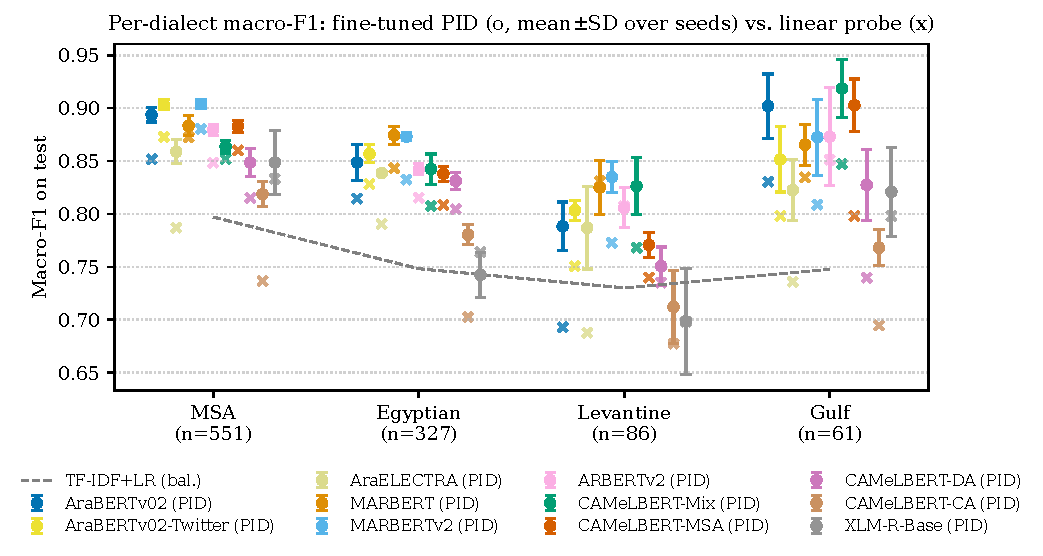
\includegraphics[width=0.9\linewidth]{figures_v2/fig1_per_dialect_forest.pdf}
\caption{Per-dialect test macro-F1 under pooled fine-tuning (mean$\pm$SD over five seeds) and the trained linear probe for the same encoder; dashed line: balanced TF-IDF.}
\label{fig:forest}
\end{figure}

\begin{table}[tbp]
\caption{Linear probes: test HM-F1 of the last-layer mean-pooled and [CLS] probes, and of the best layer selected on dev for each pooling, compared with fully fine-tuned PID HM-F1. $C$ grid: \{\probeCgrid\}.}
\label{tab:probe_layers}
\centering
\footnotesize
\adjustbox{max width=\linewidth}{\begin{tabular}{lcc|cc|cc|c}
\toprule
 & \multicolumn{2}{c|}{\textbf{Final layer}} & \multicolumn{2}{c|}{\textbf{Best layer (dev), mean}} & \multicolumn{2}{c|}{\textbf{Best layer (dev), CLS}} & \\
\textbf{Encoder} & Mean & CLS & Layer & HM & Layer & HM & FT PID HM \\
\midrule
AraBERTv02 & 0.792 & 0.806 & 7 & 0.802 & 8 & 0.781 & 0.855 \\
AraBERTv02-Twitter & 0.810 & 0.817 & 12 & 0.810 & 9 & 0.828 & 0.852 \\
AraELECTRA & 0.748 & 0.709 & 9 & 0.799 & 10 & 0.776 & 0.825 \\
MARBERT & 0.845 & 0.816 & 11 & 0.852 & 12 & 0.816 & 0.861 \\
MARBERTv2 & 0.822 & 0.818 & 9 & 0.857 & 7 & 0.835 & 0.870 \\
ARBERTv2 & 0.830 & 0.805 & 5 & 0.803 & 3 & 0.779 & 0.849 \\
CAMeLBERT-Mix & 0.817 & 0.791 & 9 & 0.808 & 12 & 0.791 & 0.861 \\
CAMeLBERT-MSA & 0.799 & 0.785 & 8 & 0.805 & 6 & 0.790 & 0.845 \\
CAMeLBERT-DA & 0.772 & 0.754 & 4 & 0.764 & 12 & 0.754 & 0.812 \\
CAMeLBERT-CA & 0.702 & 0.629 & 5 & 0.727 & 1 & 0.648 & 0.768 \\
XLM-R-Base & 0.770 & 0.753 & 12 & 0.770 & 8 & 0.751 & 0.772 \\
\bottomrule
\end{tabular}
}
\end{table}

\textbf{Fine-tuned encoders.} Full fine-tuning improves every Arabic encoder over its probe (Fig.~\ref{fig:forest}). Under PID, \bestEnc{} obtains the highest HM-F1 (\bestEncHM{} [\bestEncHMlo, \bestEncHMhi]), as well as the highest pooled F1 (\bestPoolF) and WD-F1 (\bestWdF). These differences are small relative to test-set uncertainty: the \topGroupN{} encoders \topGroup{} are not credibly below the best, and no pairwise HM-F1 or WD-F1 interval within this group excludes zero. AraELECTRA (\pidHMAraELECTRA), CAMeLBERT-DA (\pidHMCAMeLBERTDA), CAMeLBERT-CA (\pidHMCAMeLBERTCA) and XLM-R (\pidHMXLMRBase) are credibly below \bestEnc{}, and \notAboveTfidf{} are not credibly above the TF-IDF baseline (HM-F1 \tfidfHM). Pooled accuracy and dialect evenness still rank encoders differently: CAMeLBERT-Mix has one of the lowest pooled F1 of these encoders (0.858) but the smallest MSA gap and the same HM-F1 as MARBERT (0.861). The multilingual XLM-R is clearly weaker (pooled 0.803, HM-F1 0.772, WD-F1 0.694). Class-weighted training (PID-w) changes HM-F1 by at most \pidwMaxAbs{} for any encoder (Appendix Table~\ref{tab:pidw}), so the unweighted PID models are used throughout.

\textbf{LLMs.} Table~\ref{tab:llm} reports all LLM settings. With the uncalibrated 0.5 threshold, several LLMs over-predict one class, which depresses dialect F1 (AceGPT zero-shot reaches only 0.637 on Gulf); calibrating the threshold on dev improves all four zero-shot LLMs, whereas providing eight exemplars improves AceGPT and Fanar but lowers ALLaM-7B HM-F1 from 0.798 to 0.779 (and significantly lowers its pooled F1 by 0.024). All four 8-shot LLMs exceed the TF-IDF baseline in point estimate (with paired 95\% intervals excluding TF-IDF for Fanar, Qwen2.5 and AceGPT, while overlapping for ALLaM). The strongest LLM, Fanar-1-9B-Instruct (0.849 HM-F1), ties ARBERTv2 in point estimate, statistically ties the top nine encoders and significantly outperforms CAMeLBERT-CA and XLM-R-Base, trailing MARBERTv2 by 0.021 HM-F1 (95\% CI $[-0.064, +0.020]$); with eight exemplars the other three LLMs are 0.041--0.091 HM-F1 below the best encoder (intervals excluding zero for AceGPT and ALLaM). Like the encoders, every LLM is weakest on Levantine or Gulf. Few-shot prompting is therefore a competitive alternative when no labelled data exist, but none of the 7--9B LLMs surpasses the strongest fine-tuned Arabic encoders trained on 3,436 tweets.

\begin{table}[tbp]
\caption{Instruction-tuned LLMs on the leak-free test set: zero-shot (threshold 0.5), zero-shot with a dev-selected threshold, and 8-shot (one positive and one negative exemplar per dialect; mean over three exemplar draws). Last column: HM-F1 difference to the best fine-tuned encoder (PID) with 95\% paired bootstrap interval.}
\label{tab:llm}
\centering
\footnotesize
\setlength{\tabcolsep}{2.6pt}
\adjustbox{max width=\linewidth}{\begin{tabular}{llccccccc|c}
\toprule
\textbf{LLM} & \textbf{Setting} & Pooled & MSA & EGY & LEV & GLF & HM-F1 [95\% CI] & WD & $\Delta$HM vs best encoder \\
\midrule
AceGPT-v2-8B-Chat & zero-shot & 0.817 & 0.865 & 0.791 & 0.730 & 0.637 & 0.746 {\scriptsize[0.69,0.79]} & 0.637 & -- \\
AceGPT-v2-8B-Chat & zero-shot, dev threshold & 0.868 & 0.902 & 0.850 & 0.769 & 0.762 & 0.817 {\scriptsize[0.76,0.86]} & 0.762 & -0.053 {\scriptsize[-0.108, -0.009]} \\
AceGPT-v2-8B-Chat & 8-shot (3 draws) & 0.860 & 0.899 & 0.828 & 0.804 & 0.762 & 0.820 {\scriptsize[0.77,0.86]} & 0.762 & -0.050 {\scriptsize[-0.104, -0.005]} \\
\midrule
ALLaM-7B-Instruct & zero-shot & 0.846 & 0.874 & 0.836 & 0.792 & 0.710 & 0.798 {\scriptsize[0.74,0.84]} & 0.710 & -- \\
ALLaM-7B-Instruct & zero-shot, dev threshold & 0.866 & 0.903 & 0.849 & 0.779 & 0.732 & 0.811 {\scriptsize[0.76,0.85]} & 0.732 & -0.059 {\scriptsize[-0.112, -0.014]} \\
ALLaM-7B-Instruct & 8-shot (3 draws) & 0.822 & 0.851 & 0.808 & 0.777 & 0.699 & 0.779 {\scriptsize[0.72,0.82]} & 0.699 & -0.091 {\scriptsize[-0.146, -0.044]} \\
\midrule
Fanar-1-9B-Instruct & zero-shot & 0.879 & 0.915 & 0.860 & 0.777 & 0.798 & 0.834 {\scriptsize[0.78,0.87]} & 0.777 & -- \\
Fanar-1-9B-Instruct & zero-shot, dev threshold & 0.886 & 0.908 & 0.882 & 0.819 & 0.809 & 0.852 {\scriptsize[0.81,0.89]} & 0.809 & -0.018 {\scriptsize[-0.067, +0.024]} \\
Fanar-1-9B-Instruct & 8-shot (3 draws) & 0.880 & 0.906 & 0.861 & 0.819 & 0.816 & 0.849 {\scriptsize[0.80,0.88]} & 0.811 & -0.021 {\scriptsize[-0.064, +0.020]} \\
\midrule
Qwen2.5-7B-Instruct & zero-shot & 0.869 & 0.897 & 0.853 & 0.768 & 0.825 & 0.833 {\scriptsize[0.78,0.87]} & 0.768 & -- \\
Qwen2.5-7B-Instruct & zero-shot, dev threshold & 0.868 & 0.897 & 0.852 & 0.768 & 0.820 & 0.831 {\scriptsize[0.78,0.87]} & 0.768 & -0.039 {\scriptsize[-0.090, +0.007]} \\
Qwen2.5-7B-Instruct & 8-shot (3 draws) & 0.862 & 0.897 & 0.832 & 0.749 & 0.852 & 0.829 {\scriptsize[0.78,0.86]} & 0.749 & -0.041 {\scriptsize[-0.089, +0.006]} \\
\bottomrule
\end{tabular}
}
\end{table}

\textbf{Which dialects are hard?} Levantine is the worst dialect for every fine-tuned encoder (\levWorstN{} of \nEnc) despite having more training data than Gulf (239 vs.\ 184 tweets). The mixed model (Table~\ref{tab:glmm}) quantifies this over all \glmmNmodels{} encoders while accounting for tweet difficulty and fertility: relative to MSA, the Levantine effect is negative for every encoder and its 95\% credible interval excludes zero for \glmmNegLEV{} of them; Egyptian is credibly harder for \glmmNegEGY{} encoders and Gulf for \glmmNegGLF. The tweet random effect is large (Table~\ref{tab:glmm}), i.e.\ errors concentrate on the same hard tweets across encoders, which is why instance-level paired tests are needed. After Holm correction over 30 pooled and per-dialect McNemar tests (Table~\ref{tab:mcnemar}), only six comparisons are significant, all against XLM-R (pooled and on Egyptian); no difference among AraBERTv02, MARBERT and CAMeLBERT-Mix survives.

\begin{table}[tbp]
\caption{McNemar tests on seed-ensembled (majority-vote) PID predictions: $b$/$c$ = tweets only A / only B classifies correctly. $^*$Holm-adjusted $p<0.05$ over all 30 tests.}
\label{tab:mcnemar}
\centering
\footnotesize
\adjustbox{max width=\linewidth}{\begin{tabular}{lccccc}
\toprule
\textbf{Pair (A vs B)} & \textbf{All} & \textbf{MSA} & \textbf{EGY} & \textbf{LEV} & \textbf{GLF} \\
\midrule
MARBERT vs XLM-R-Base & 95/42$^*$ & 35/26 & 44/10$^*$ & 12/3 & 4/3 \\
AraBERTv02 vs XLM-R-Base & 88/37$^*$ & 32/22 & 40/10$^*$ & 12/4 & 4/1 \\
CAMeLBERT-Mix vs XLM-R-Base & 83/44$^*$ & 29/29 & 37/11$^*$ & 13/4 & 4/0 \\
AraBERTv02 vs CAMeLBERT-Mix & 38/26 & 21/11 & 14/10 & 2/3 & 1/2 \\
MARBERT vs CAMeLBERT-Mix & 47/33 & 29/20 & 14/6 & 4/4 & 0/3 \\
AraBERTv02 vs MARBERT & 36/38 & 19/18 & 10/14 & 3/4 & 4/2 \\
\bottomrule
\end{tabular}
}
\end{table}

\begin{table}[tbp]
\caption{Bayesian beta-binomial mixed model of per-tweet correctness under PID: dialect effects (log-odds of a correct prediction relative to MSA, i.e.\ $b_d+g_{m,d}$) per encoder, posterior mean with 95\% credible interval ($^*$: interval excludes zero). The fertility coefficient is per standard deviation within encoder $\times$ dialect.}
\label{tab:glmm}
\centering
\footnotesize
\adjustbox{max width=\linewidth}{\begin{tabular}{lccc}
\toprule
\textbf{Encoder (PID)} & EGY vs MSA & LEV vs MSA & GLF vs MSA \\
\midrule
AraBERTv02 & -0.62 {\scriptsize[-1.21,-0.03]}$^*$ & -1.63 {\scriptsize[-2.49,-0.78]}$^*$ & -0.69 {\scriptsize[-1.73,+0.35]} \\
AraBERTv02-Twitter & -0.67 {\scriptsize[-1.35,+0.01]} & -1.52 {\scriptsize[-2.54,-0.51]}$^*$ & -1.25 {\scriptsize[-2.38,-0.08]}$^*$ \\
AraELECTRA & -0.16 {\scriptsize[-0.80,+0.48]} & -1.26 {\scriptsize[-2.21,-0.28]}$^*$ & -0.70 {\scriptsize[-1.84,+0.45]} \\
MARBERT & -0.12 {\scriptsize[-0.78,+0.53]} & -0.91 {\scriptsize[-1.90,+0.10]} & -0.53 {\scriptsize[-1.69,+0.69]} \\
MARBERTv2 & -0.33 {\scriptsize[-1.01,+0.33]} & -1.24 {\scriptsize[-2.31,-0.17]}$^*$ & -1.05 {\scriptsize[-2.21,+0.14]} \\
ARBERTv2 & -0.59 {\scriptsize[-1.22,+0.08]} & -1.20 {\scriptsize[-2.16,-0.22]}$^*$ & -0.74 {\scriptsize[-1.88,+0.42]} \\
CAMeLBERT-Mix & -0.09 {\scriptsize[-0.72,+0.55]} & -0.60 {\scriptsize[-1.61,+0.43]} & +0.42 {\scriptsize[-0.80,+1.70]} \\
CAMeLBERT-MSA & -0.53 {\scriptsize[-1.18,+0.11]} & -1.60 {\scriptsize[-2.58,-0.59]}$^*$ & -0.51 {\scriptsize[-1.67,+0.76]} \\
CAMeLBERT-DA & -0.05 {\scriptsize[-0.68,+0.59]} & -1.22 {\scriptsize[-2.15,-0.28]}$^*$ & -0.51 {\scriptsize[-1.65,+0.66]} \\
CAMeLBERT-CA & -0.28 {\scriptsize[-0.88,+0.33]} & -1.03 {\scriptsize[-1.96,-0.08]}$^*$ & -0.72 {\scriptsize[-1.75,+0.36]} \\
XLM-R-Base & -0.96 {\scriptsize[-1.56,-0.35]}$^*$ & -1.61 {\scriptsize[-2.50,-0.68]}$^*$ & -0.84 {\scriptsize[-1.89,+0.25]} \\
\midrule
\multicolumn{4}{l}{Fertility (per SD, within encoder$\times$dialect): -0.028 [-0.205, +0.140];\ $\sigma_{\text{tweet}}$ = 3.12} \\
\multicolumn{4}{l}{4 chains $\times$ 1000 draws; max $\hat R$ = 1.010; min bulk ESS = 519; divergences = 0} \\
\bottomrule
\end{tabular}
}
\end{table}

\textbf{How uncertain is HM-F1?} Because HM-F1 is dominated by the weakest dialects, its uncertainty is dominated by the two smallest test sets. The bootstrap SD of HM-F1 is \hmSdMin--\hmSdMax{} for every encoder, larger than that of pooled F1 (at most \pooledSdMax), and a first-order (delta-method) decomposition attributes \levGlfShareMin--\levGlfShareMax\% of its variance to Levantine and Gulf (Table~\ref{tab:hm_variance}), whose 86 and 61 test tweets give per-dialect F1 SDs of about 0.04--0.05. HM-F1 is therefore the right quantity to report for robustness, but it needs intervals, and with test sets of this size only differences of several points are resolvable.

\begin{table}[tbp]
\caption{Uncertainty of HM-F1 under PID: bootstrap SD of pooled F1, HM-F1 and each dialect's F1, and each dialect's first-order share of the bootstrap variance of HM-F1.}
\label{tab:hm_variance}
\centering
\footnotesize
\setlength{\tabcolsep}{3pt}
\adjustbox{max width=\linewidth}{\begin{tabular}{lcc|cccc|cccc}
\toprule
 & & & \multicolumn{4}{c|}{\textbf{Bootstrap SD of dialect F1}} & \multicolumn{4}{c}{\textbf{Share of Var(HM) (\%)}} \\
\textbf{Encoder (PID)} & SD pooled & SD HM & MSA & EGY & LEV & GLF & MSA & EGY & LEV & GLF \\
\midrule
AraBERTv02 & 0.011 & 0.018 & 0.014 & 0.022 & 0.045 & 0.037 & 3 & 10 & 60 & 26 \\
AraBERTv02-Twitter & 0.010 & 0.019 & 0.013 & 0.020 & 0.047 & 0.049 & 2 & 7 & 49 & 43 \\
AraELECTRA & 0.013 & 0.021 & 0.016 & 0.022 & 0.049 & 0.054 & 4 & 7 & 45 & 44 \\
MARBERT & 0.010 & 0.018 & 0.014 & 0.019 & 0.045 & 0.046 & 3 & 6 & 49 & 42 \\
MARBERTv2 & 0.010 & 0.017 & 0.013 & 0.020 & 0.044 & 0.045 & 3 & 7 & 48 & 42 \\
ARBERTv2 & 0.011 & 0.017 & 0.014 & 0.020 & 0.045 & 0.044 & 3 & 8 & 53 & 35 \\
CAMeLBERT-Mix & 0.011 & 0.017 & 0.015 & 0.022 & 0.044 & 0.038 & 5 & 13 & 55 & 27 \\
CAMeLBERT-MSA & 0.011 & 0.019 & 0.015 & 0.022 & 0.049 & 0.039 & 3 & 9 & 66 & 23 \\
CAMeLBERT-DA & 0.013 & 0.021 & 0.017 & 0.022 & 0.050 & 0.053 & 3 & 7 & 50 & 39 \\
CAMeLBERT-CA & 0.012 & 0.021 & 0.016 & 0.022 & 0.049 & 0.051 & 3 & 8 & 49 & 41 \\
XLM-R-Base & 0.015 & 0.023 & 0.019 & 0.025 & 0.051 & 0.051 & 6 & 10 & 53 & 31 \\
\bottomrule
\end{tabular}
}
\end{table}

\subsection{Cross-Dialect Transfer (RQ2)}
\label{sec:res_transfer}
\textbf{Leaving the target dialect out.} Table~\ref{tab:tost} compares each transfer regime with a pooled control trained on the same number of tweets drawn from all four dialects. For the \nArab{} Arabic encoders LODO changes HM-F1 by \lodoArDeltaMin{} to \lodoArDeltaMax{}, and \lodoArSig{} of their intervals exclude zero; the multilingual XLM-R is the exception, with a change of \xlmLodo{} HM-F1 [90\% CI \xlmLodoLo, \xlmLodoHi]. Most of the apparent LODO ``drop'' relative to full PID is a training-size effect, which the size-matched controls remove.

\textbf{Is ``no detectable loss'' evidence of no loss?} Not by itself. With the pre-stated margin of $\pm0.02$ HM-F1, only \nLodoEquiv{} of \nLodoModels{} encoders is formally equivalent under LODO: the 90\% intervals have half-widths of about 0.02--0.03, and the minimum detectable effect is \lodoMdeMin--\lodoMdeMax{} HM-F1. What the data do support is a bound: for every Arabic encoder the 90\% interval excludes LODO losses larger than \lodoArLossBound{} HM-F1 (and MSA-only losses larger than \msaArLossBound). At the level of a single dialect the study is much less sensitive (MDE \lodoMdeLevMin--\lodoMdeLevMax{} on Levantine and \lodoMdeGlfMin--\lodoMdeGlfMax{} on Gulf), so per-dialect transfer changes below roughly 0.07--0.10 cannot be resolved, and single-dialect TOST at $\pm0.05$ passes for only 14 of 33 LODO and 13 of 33 MSA-only cells because the margin lies below most single-dialect MDEs.

\begin{table}[tbp]
\caption{Transfer equivalence: change in HM-F1 of LODO relative to the pooled control trained on 1,531 tweets and of MSA-only relative to the pooled control trained on 1,905 tweets (mean over five seeds), 90\% hierarchical bootstrap interval, TOST equivalence at $\pm0.02$ (\textbf{Yes}), and minimum detectable effect (80\% power) for HM-F1 and for single-dialect F1 on Gulf and Levantine.}
\label{tab:tost}
\centering
\footnotesize
\setlength{\tabcolsep}{3pt}
\adjustbox{max width=\linewidth}{\begin{tabular}{lcccc|cccc|cc}
\toprule
 & \multicolumn{4}{c|}{\textbf{LODO $-$ Pooled(1,531)}} & \multicolumn{4}{c|}{\textbf{MSA-only $-$ Pooled(1,905)}} & \multicolumn{2}{c}{\textbf{MDE (LODO)}} \\
\textbf{Encoder} & $\Delta$HM & 90\% CI & Eq. & MDE & $\Delta$HM & 90\% CI & Eq. & MDE & GLF & LEV \\
\midrule
AraBERTv02 & -0.002 & {\scriptsize[-0.018, +0.015]} & \cmark & 0.029 & -0.005 & {\scriptsize[-0.028, +0.018]} &  & 0.040 & 0.075 & 0.069 \\
AraBERTv02-Twitter & -0.009 & {\scriptsize[-0.025, +0.007]} &  & 0.027 & +0.003 & {\scriptsize[-0.015, +0.021]} &  & 0.032 & 0.088 & 0.069 \\
AraELECTRA & -0.015 & {\scriptsize[-0.037, +0.006]} &  & 0.037 & -0.001 & {\scriptsize[-0.023, +0.018]} &  & 0.035 & 0.107 & 0.059 \\
MARBERT & -0.000 & {\scriptsize[-0.022, +0.019]} &  & 0.035 & -0.005 & {\scriptsize[-0.026, +0.015]} &  & 0.035 & 0.095 & 0.064 \\
MARBERTv2 & +0.005 & {\scriptsize[-0.014, +0.024]} &  & 0.033 & -0.013 & {\scriptsize[-0.033, +0.007]} &  & 0.035 & 0.096 & 0.052 \\
ARBERTv2 & -0.010 & {\scriptsize[-0.035, +0.013]} &  & 0.041 & +0.001 & {\scriptsize[-0.027, +0.031]} &  & 0.049 & 0.108 & 0.073 \\
CAMeLBERT-Mix & +0.008 & {\scriptsize[-0.016, +0.032]} &  & 0.042 & -0.006 & {\scriptsize[-0.031, +0.017]} &  & 0.042 & 0.124 & 0.077 \\
CAMeLBERT-MSA & +0.004 & {\scriptsize[-0.014, +0.022]} &  & 0.031 & -0.009 & {\scriptsize[-0.030, +0.011]} &  & 0.035 & 0.101 & 0.046 \\
CAMeLBERT-DA & -0.011 & {\scriptsize[-0.028, +0.006]} &  & 0.029 & +0.009 & {\scriptsize[-0.011, +0.031]} &  & 0.036 & 0.078 & 0.050 \\
CAMeLBERT-CA & -0.011 & {\scriptsize[-0.045, +0.021]} &  & 0.056 & +0.004 & {\scriptsize[-0.029, +0.038]} &  & 0.057 & 0.112 & 0.114 \\
XLM-R-Base & -0.059 & {\scriptsize[-0.091, -0.030]} &  & 0.052 & -0.011 & {\scriptsize[-0.039, +0.018]} &  & 0.049 & 0.137 & 0.127 \\
\bottomrule
\end{tabular}
}
\end{table}

\textbf{MSA-only training.} Against a pooled control of the same size, MSA-only training changes HM-F1 by \msaDeltaMin{} to \msaDeltaMax{}, and \nMsaSig{} of \nLodoModels{} intervals exclude zero. Per-dialect point estimates suggest that the MSA-only cost, if any, falls on Gulf (\msaGlfLossN{} of \nEnc{} encoders lose Gulf F1), but these changes are below the per-dialect MDE. Absolute per-dialect scores for all regimes are shown in Fig.~\ref{fig:transfer}.

\begin{figure}[t]
\centering
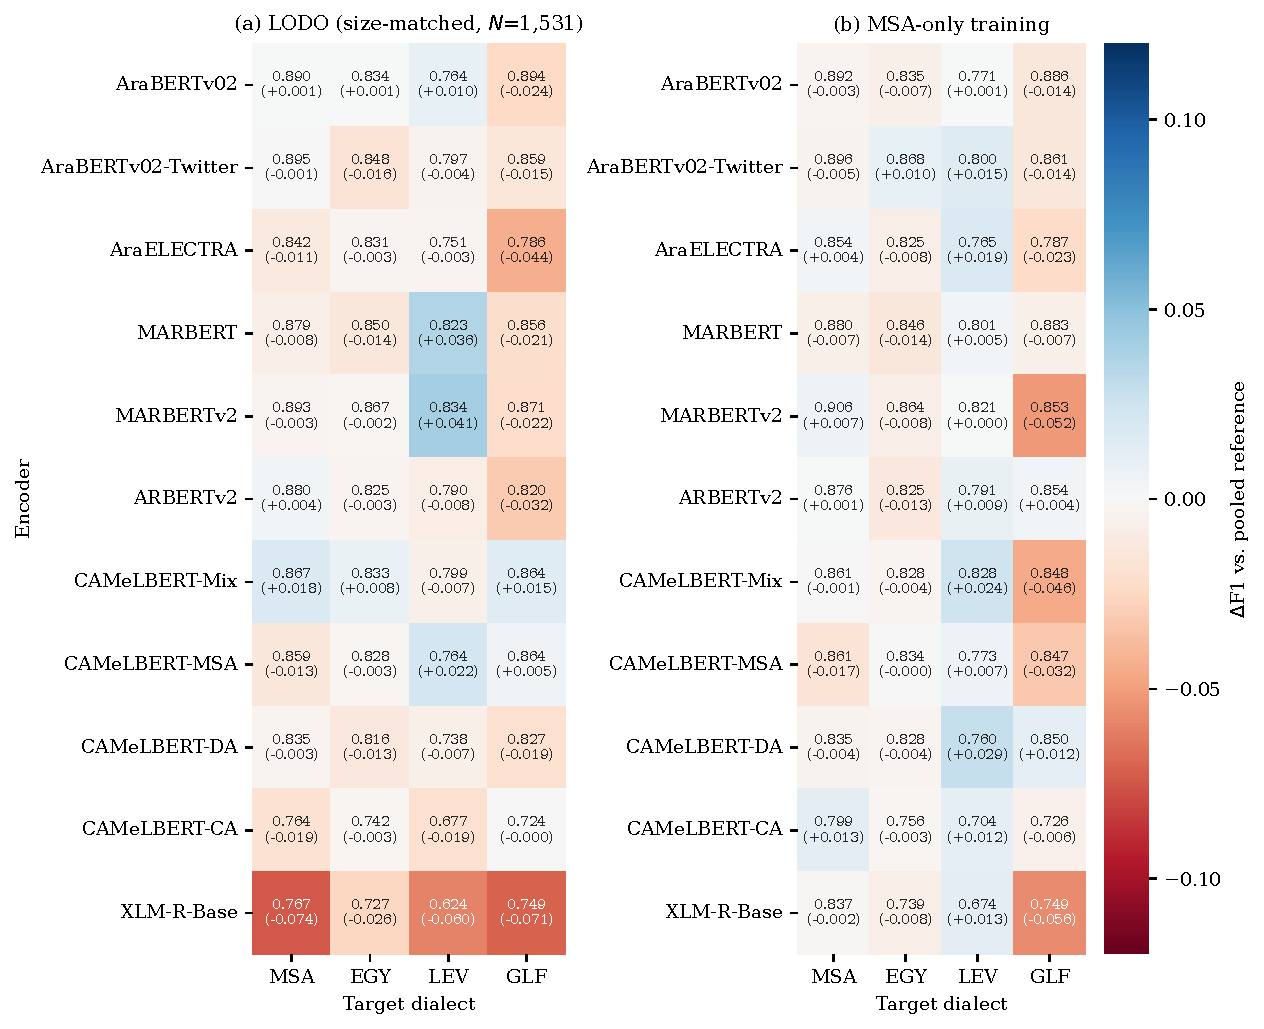
\includegraphics[width=\linewidth]{figures_v2/fig2_transfer_drop_heatmap.pdf}
\caption{Target-dialect macro-F1 (and change relative to the size-matched pooled control) for all encoders under (a) size-matched leave-one-dialect-out training and (b) MSA-only training.}
\label{fig:transfer}
\end{figure}

\textbf{How much in-dialect data helps.} Fig.~\ref{fig:lc} and Table~\ref{tab:lc} add increasing amounts of target-dialect data to the LODO training set. Adding in-dialect tweets yields no statistically detectable gain for the Arabic encoders: with all target-dialect training tweets added, the change relative to LODO ranges from \lcGainAllMin{} to \lcGainAllMax{}, and \lcSigAll{} of the \lcCells{} encoder $\times$ dialect intervals exclude zero, at this or any smaller $k$. XLM-R-Base exhibits an upward point-estimate trajectory on Levantine ($-0.032$ at $k=25$ to $+0.068$ at $k=\mathrm{all}$) and Gulf ($+0.046$ at $k=\mathrm{all}$) that remains within the wide single-dialect MDEs. For the Arabic encoders the result is consistent with the transfer analysis: without in-dialect data, they already perform about as well as with it.

\begin{figure}[t]
\centering
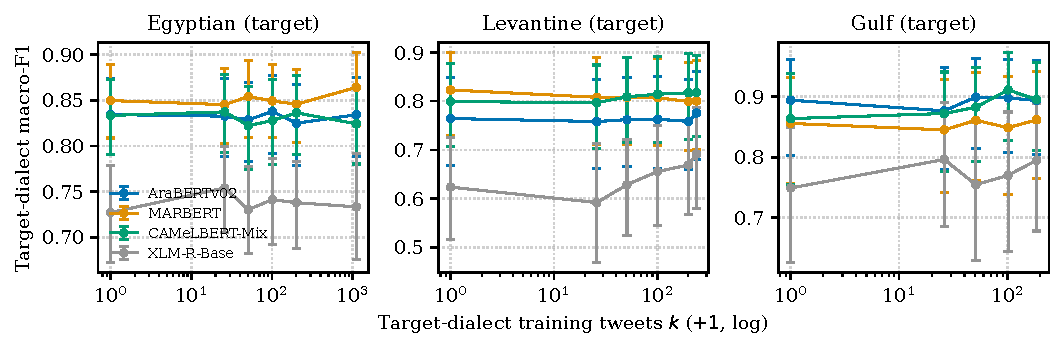
\includegraphics[width=\linewidth]{figures_v2/fig5_learning_curve.pdf}
\caption{Learning curve: target-dialect macro-F1 when $k$ target-dialect tweets are added to the size-matched LODO training set ($k{=}0$ is LODO); mean over five seeds with 95\% hierarchical bootstrap intervals.}
\label{fig:lc}
\end{figure}

\begin{table}[tbp]
\caption{Learning curve: target-dialect F1 at $k{=}0$ (LODO) and gain from adding $k$ target-dialect tweets (mean over five seeds; $^*$: 95\% interval of the gain excludes zero).}
\label{tab:lc}
\centering
\footnotesize
\adjustbox{max width=\linewidth}{\begin{tabular}{llcccccc|c}
\toprule
\textbf{Target} & \textbf{Encoder} & $k{=}0$ F1 & $\Delta k{=}25$ & $\Delta k{=}50$ & $\Delta k{=}100$ & $\Delta k{=}200$ & $\Delta k{=}all$ & $N_{\text{all}}$ \\
\midrule
EGY & AraBERTv02 & 0.834 & -0.002 & -0.006 & +0.003 & -0.009 & -0.000 & 1108 \\
EGY & MARBERT & 0.850 & -0.004 & +0.004 & -0.000 & -0.004 & +0.014 & 1108 \\
EGY & CAMeLBERT-Mix & 0.833 & +0.004 & -0.011 & -0.006 & +0.003 & -0.009 & 1108 \\
EGY & XLM-R-Base & 0.727 & +0.027 & +0.003 & +0.014 & +0.011 & +0.006 & 1108 \\
LEV & AraBERTv02 & 0.764 & -0.006 & -0.002 & -0.001 & -0.006 & +0.012 & 239 \\
LEV & MARBERT & 0.823 & -0.015 & -0.015 & -0.016 & -0.024 & -0.023 & 239 \\
LEV & CAMeLBERT-Mix & 0.799 & -0.002 & +0.010 & +0.015 & +0.018 & +0.019 & 239 \\
LEV & XLM-R-Base & 0.624 & -0.032 & +0.005 & +0.032 & +0.045 & +0.068 & 239 \\
GLF & AraBERTv02 & 0.894 & -0.018 & +0.005 & +0.004 & -- & -0.001 & 184 \\
GLF & MARBERT & 0.856 & -0.011 & +0.005 & -0.007 & -- & +0.006 & 184 \\
GLF & CAMeLBERT-Mix & 0.864 & +0.008 & +0.019 & +0.047 & -- & +0.031 & 184 \\
GLF & XLM-R-Base & 0.749 & +0.047 & +0.006 & +0.021 & -- & +0.046 & 184 \\
\bottomrule
\end{tabular}
}
\end{table}

\subsection{Replication on ArSarcasm-v2}
\label{sec:res_v2}
Table~\ref{tab:v2} repeats the transfer protocol on ArSarcasm-v2. Under PID the ordering resembles the main corpus: MARBERTv2 has the highest three-dialect HM-F1 (0.814) and XLM-R the lowest (0.737). Relative to their size-matched pooled controls, LODO changes HM-F1 by \vLodoDeltaMin{} to \vLodoDeltaMax{} and MSA-only training by \vMsaDeltaMin{} to \vMsaDeltaMax{}; \vLodoSig{} and \vMsaSig{} of the \vModels{} intervals, respectively, exclude zero. The main transfer finding for Arabic encoders therefore replicates on an independent test set. XLM-R's LODO loss does not: on v2 its LODO change is $+0.022$ [$-0.022$, $+0.067$], so the XLM-R result should be regarded as corpus-specific. Levantine (28 test tweets, one positive) is shown only descriptively.

\begin{table}[tbp]
\caption{ArSarcasm-v2 replication (binary sentiment; mean over five seeds). Dialect profile over MSA, Egyptian and Gulf (Levantine test: 28 tweets, one positive; reported descriptively only). $\Delta$HM: LODO and MSA-only relative to their size-matched pooled controls, with 95\% interval. LEV$^\ddagger$ has 28 test tweets (one positive) and is excluded from HM3. Intervals are 95\% hierarchical bootstrap CIs (whereas Table~\ref{tab:tost} reports 90\% CIs corresponding to two one-sided $\alpha=0.05$ TOST tests).}
\label{tab:v2}
\centering
\footnotesize
\setlength{\tabcolsep}{3pt}
\adjustbox{max width=\linewidth}{\begin{tabular}{lcccccc|cc}
\toprule
\textbf{System} & Pooled & MSA & EGY & GLF & HM$_3$ [95\% CI] & LEV$^\ddagger$ & $\Delta$HM LODO & $\Delta$HM MSA-only \\
\midrule
Majority & 0.426 & 0.422 & 0.477 & 0.402 & 0.432 & -- & -- & -- \\
\midrule
AraBERTv02 & 0.810 & 0.813 & 0.726 & 0.793 & 0.775 {\scriptsize[0.73,0.81]} & 1.00 & -0.013 {\scriptsize[-0.033, +0.008]} & +0.018 {\scriptsize[-0.005, +0.043]} \\
MARBERT & 0.820 & 0.819 & 0.759 & 0.817 & 0.797 {\scriptsize[0.76,0.83]} & 0.96 & +0.004 {\scriptsize[-0.022, +0.030]} & -0.007 {\scriptsize[-0.029, +0.014]} \\
MARBERTv2 & 0.825 & 0.824 & 0.803 & 0.816 & 0.814 {\scriptsize[0.77,0.85]} & 0.83 & -0.000 {\scriptsize[-0.026, +0.029]} & -0.020 {\scriptsize[-0.052, +0.008]} \\
CAMeLBERT-Mix & 0.790 & 0.789 & 0.723 & 0.790 & 0.766 {\scriptsize[0.72,0.80]} & 1.00 & +0.004 {\scriptsize[-0.015, +0.025]} & -0.009 {\scriptsize[-0.032, +0.017]} \\
XLM-R-Base & 0.756 & 0.753 & 0.702 & 0.760 & 0.737 {\scriptsize[0.69,0.77]} & 0.72 & +0.022 {\scriptsize[-0.022, +0.067]} & -0.038 {\scriptsize[-0.152, +0.037]} \\
\bottomrule
\end{tabular}
}
\end{table}

\subsection{Pretraining Variant (RQ3)}
\label{sec:res_variant}
The four CAMeLBERT models share architecture and tokenizer, so differences between them isolate pretraining data. After full fine-tuning, HM-F1 is \pidHMCAMeLBERTMix{} for Mix, \pidHMCAMeLBERTMSA{} for MSA, \pidHMCAMeLBERTDA{} for DA and \pidHMCAMeLBERTCA{} for CA. Both Mix and MSA credibly exceed DA (paired hierarchical-bootstrap differences \pdCAMeLBERTMixCAMeLBERTDAHM{} and \pdCAMeLBERTMSACAMeLBERTDAHM), and DA in turn exceeds CA (\pdCAMeLBERTDACAMeLBERTCAHM), but the Mix$-$MSA difference (\pdCAMeLBERTMixCAMeLBERTMSAHM) is not significant, even though Mix has the higher WD-F1 (0.822 vs.\ 0.771) and a much smaller MSA gap. After Holm--Bonferroni correction across the six pairwise comparisons, four pairs (Mix vs.\ CA, MSA vs.\ CA, DA vs.\ CA and Mix vs.\ DA) remain statistically significant while MSA vs.\ DA ($p=0.029$ vs.\ Holm threshold $0.025$) is borderline. Because the four CAMeLBERT variants also differ in pretraining corpus size (Mix 167\,GB, MSA 107\,GB, DA 54\,GB and CA 6\,GB), corpus scale covaries with register composition and likely contributes to CA's lower performance and to MSA outperforming DA even on Gulf and Levantine test tweets. The same ordering appears in the frozen probes (HM-F1 0.817, 0.799, 0.772 and 0.702 for CA). Dialect-only and classical-only pretraining are therefore insufficient for a mixed MSA--dialect test set, and covering both registers yields the most even profile, consistent with the variant-proximity findings of \cite{inoue2021interplay}; under full fine-tuning, however, the advantage of mixed over MSA pretraining is within test-set uncertainty. Among the other same-tokenizer pairs, continued pretraining (MARBERTv2$-$MARBERT: \pdMARBERTvMARBERTHM) and additional tweet pretraining (AraBERTv02-Twitter$-$AraBERTv02: \pdAraBERTvTwitterAraBERTvHM) do not change HM-F1 credibly, whereas replacing masked-language-model pretraining by the ELECTRA objective on the same data and vocabulary lowers it slightly (AraELECTRA$-$AraBERTv02: \pdAraELECTRAAraBERTvHM; the interval only just excludes zero). The MSA-pretrained ARBERTv2, which has its own 100K vocabulary, is within uncertainty of the dialect-pretrained MARBERTv2 (\pdARBERTvMARBERTvHM), so pretraining variant matters most at the extremes (dialect-only or classical-only data), not between MSA-heavy and dialect-rich encoders.

\subsection{Dispersion-Only Robustness Metrics (RQ4)}
\label{sec:res_metric}
Table~\ref{tab:metric_validity} and Fig.~\ref{fig:metric_validity} show why a dispersion-only index should not be used to rank systems, whether it is computed on accuracy or on F1. Because per-dialect scores of any reasonable system differ by only a few points, the variance is of order $10^{-3}$ and DRI-F1 lies in [0.9945, 1.0000] for all \mvN{} systems (baselines, probes and the seed means of every fine-tuned encoder and regime). The majority classifier, which never predicts a positive tweet, is ranked \mvRankAcc{} of \mvN{} by DRI-acc and \emph{first} by DRI-F1, while its HM-F1 is the lowest. Across systems, both indices are only weakly related to HM-F1 (Kendall $\tau$=\mvTauAcc{} and \mvTauFone), whereas HM-F1 agrees with WD-F1 ($\tau$=\mvTauWd) and pooled F1 ($\tau$=\mvTauPooled) yet still separates encoders that pooled F1 conflates. Synthetic profiles make the failure explicit: a uniformly mediocre and a degenerate classifier both receive DRI-F1 1.000, the same as a uniformly strong one. Moving the index from accuracy to F1 does not help, because the problem is not the per-dialect score but the absence of the level: dispersion is informative only together with level, which HM-F1 and WD-F1 provide.

\begin{table}[tbp]
\caption{Dispersion-only indices versus level-aware metrics. Synthetic per-dialect F1 profiles (top) and empirical systems (bottom). F1$^*$ is the dialect mean for synthetic and pooled macro-F1 for empirical rows; DRI $=1/(1+\operatorname{Var}_d)$ of per-dialect accuracy (DRI-acc) or F1 (DRI-F1). Empirical DRI values are computed per seed and averaged across the five seeds (which explains why MARBERTv2's mean per-seed DRI-F1 is 0.9991 whereas computing DRI on seed-averaged dialect F1s gives 0.9994).}
\label{tab:metric_validity}
\centering
\footnotesize
\setlength{\tabcolsep}{3pt}
\adjustbox{max width=\linewidth}{\begin{tabular}{lcccccc}
\toprule
\textbf{Profile} & \textbf{F1}$^*$ & \textbf{HM-F1} & \textbf{WD-F1} & \textbf{Gap} & \textbf{DRI-acc} & \textbf{DRI-F1} \\
\midrule
Ideal uniform high & 0.850 & 0.850 & 0.850 & 0.000 & -- & 1.0000 \\
Strong, slightly uneven & 0.835 & 0.834 & 0.800 & 0.080 & -- & 0.9991 \\
MSA-biased drop & 0.750 & 0.736 & 0.620 & 0.280 & -- & 0.9894 \\
Uniform mediocre & 0.550 & 0.550 & 0.550 & 0.000 & -- & 1.0000 \\
Degenerate majority & 0.409 & 0.409 & 0.402 & 0.000 & -- & 1.0000 \\
\midrule
Majority (empirical) & 0.409 & 0.409 & 0.402 & 0.000 & 0.9996 & 1.0000 \\
TF-IDF+LR (empirical) & 0.773 & 0.755 & 0.730 & 0.067 & 0.9995 & 0.9994 \\
MARBERTv2 PID (empirical) & 0.888 & 0.870 & 0.833 & 0.071 & 0.9995 & 0.9991 \\
\midrule
\multicolumn{7}{l}{Rank of Majority among 79 systems: HM-F1 79, DRI-acc 7, DRI-F1 1} \\
\multicolumn{7}{l}{Kendall $\tau$ with HM-F1: pooled 0.86, WD 0.75, DRI-acc 0.22, DRI-F1 0.18} \\
\bottomrule
\end{tabular}
}
\end{table}

\begin{figure}[t]
\centering
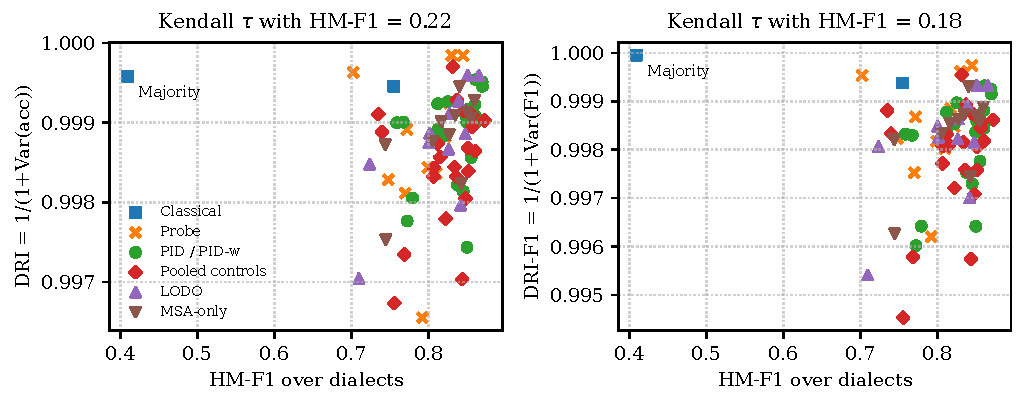
\includegraphics[width=\linewidth]{figures_v2/fig4_metric_validity.pdf}
\caption{Dispersion-only indices on (a) accuracy and (b) F1 versus HM-F1 for all evaluated systems (seed means). Both indices place the majority classifier at or near the top.}
\label{fig:metric_validity}
\end{figure}

\subsection{Sarcasm, Orthography and Tokenization (RQ4)}
\label{sec:error_analysis}
\textbf{Sarcasm.} Macro-F1 appears to collapse on sarcastic tweets (0.82--0.89 on non-sarcastic vs.\ 0.54--0.67 on sarcastic tweets across the \nEnc{} encoders; Table~\ref{tab:sarcasm} shows the four core encoders), but this gap is mainly an artefact of class composition: 294 of the 306 sarcastic test tweets are negative, so the positive class has only 12 instances and dominates macro-F1. Accuracy is \emph{higher} on sarcastic tweets for every encoder, and negative-class recall is the same with or without sarcasm (all bootstrap intervals of the difference contain zero). Positive-labelled sarcastic tweets are recognized in only 2--6 of 12 cases, but with $n=12$ (MSA 5, Egyptian 3, Levantine 2 and Gulf 2) no conclusion about sarcastic positive tweets is possible. What the data do show is that per-dialect macro-F1 without controlling for class composition would wrongly attribute dialect gaps to sarcasm, which is twice as frequent in Egyptian as in MSA.

\begin{table}[tbp]
\caption{Pooled PID results on non-sarcastic / sarcastic test tweets. $\Delta$Rec.\,neg: non-sarcastic minus sarcastic negative-class recall with 95\% bootstrap interval.}
\label{tab:sarcasm}
\centering
\footnotesize
\adjustbox{max width=\linewidth}{\begin{tabular}{lccccc}
\toprule
\textbf{Encoder (PID)} & \textbf{Acc.} & \textbf{Rec.\,neg} & \textbf{Rec.\,pos} & \textbf{Macro-F1} & \textbf{$\Delta$Rec.\,neg} \\
\midrule
AraBERTv02 & 0.885/0.938 & 0.945/0.959 & 0.802/0.417 & 0.879/0.656 & -0.015 {\scriptsize[-0.046,+0.017]} \\
MARBERT & 0.893/0.925 & 0.940/0.946 & 0.828/0.417 & 0.889/0.632 & -0.006 {\scriptsize[-0.041,+0.028]} \\
CAMeLBERT-Mix & 0.869/0.935 & 0.947/0.952 & 0.762/0.500 & 0.862/0.670 & -0.005 {\scriptsize[-0.037,+0.029]} \\
XLM-R-Base & 0.835/0.889 & 0.916/0.912 & 0.723/0.333 & 0.826/0.565 & +0.004 {\scriptsize[-0.037,+0.045]} \\
\midrule
$n$ (pos.) & 719 (303) / 306 (12) & & & & \\
\bottomrule
\end{tabular}
}
\end{table}

\textbf{Orthography and length (descriptive).} After removing URLs, mentions and retweet markers, only 47 test tweets contain Latin script, 70 contain Arabic letter elongation and 126 contain emoji. Tweets with emoji or repeated punctuation have somewhat lower F1 for most encoders, and long tweets ($>$20 words) are harder than short ones ($\le$10 words) for every encoder. These analyses are \emph{descriptive}: the buckets are small, overlap with dialect and class, and are not tested formally.

\textbf{Tokenizer fertility.} MARBERT's 100K vocabulary segments the test tweets most efficiently (1.79 subwords per word on the dialects vs.\ 2.11--2.15 for AraBERTv02 and CAMeLBERT and 2.46 for XLM-R; Table~\ref{tab:models}), and across encoder--dialect pairs fertility correlates negatively with F1 (Fig.~\ref{fig:sarcasm_fertility}b). This correlation is descriptive and confounded: Levantine has the highest fertility under every tokenizer and is also the hardest dialect, and the four CAMeLBERT variants have identical fertility yet differ substantially in F1. In the mixed model, which controls for encoder, dialect, their interaction and tweet difficulty, the within-cell fertility effect is \glmmFert{} log-odds per SD [\glmmFertLo, \glmmFertHi], i.e.\ not credibly different from zero: tweets that are segmented into more subwords than other tweets of the same dialect are not harder for the same encoder. Segmentation efficiency shows no statistically detectable within-cell effect ($-0.028$ log-odds per SD, 95\% CI $[-0.205, +0.140]$).

\begin{figure}[t]
\centering
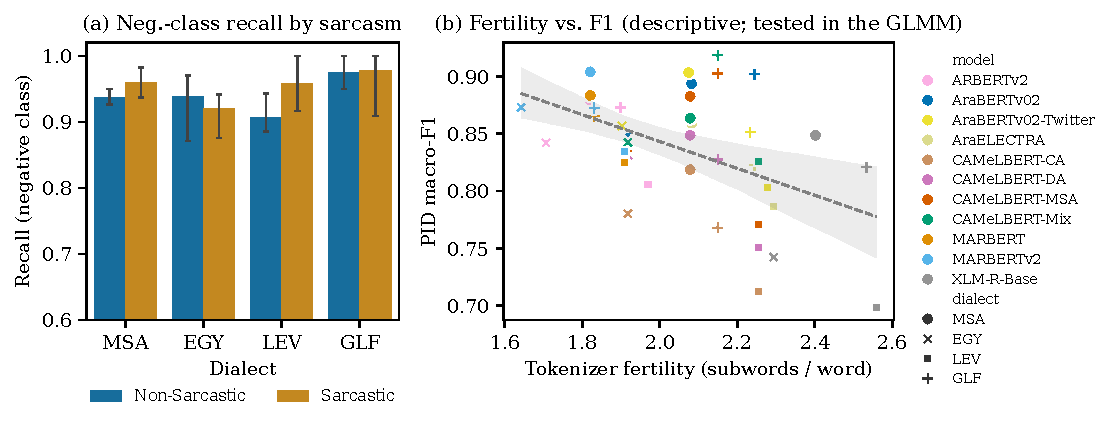
\includegraphics[width=\linewidth]{figures_v2/fig3_sarcasm_and_fertility.pdf}
\caption{(a) Negative-class recall on non-sarcastic vs.\ sarcastic tweets per dialect (bars: mean, whiskers: range over encoders). (b) Tokenizer fertility vs.\ per-dialect PID macro-F1 (descriptive; the effect is tested within encoder $\times$ dialect in the mixed model).}
\label{fig:sarcasm_fertility}
\end{figure}

\subsection{Three-Class Replication}
\label{sec:res_threeclass}
Repeating pooled fine-tuning with all three sentiment classes for the four core encoders (10,132 unique tweets; 6,813 training, 1,203 development and 2,089 test tweets) preserves the main binary findings (Table~\ref{tab:three_class}): MARBERT is best (pooled 0.725, HM-F1 0.656), Arabic-specific encoders are ahead of XLM-R (0.686, 0.616), and Levantine is again the weakest dialect for three of the four encoders. The three-class results are, however, confounded by class composition: the neutral class makes up 61\% of MSA test tweets but far less of each dialect, so per-dialect macro-F1 differences mix dialect difficulty with neutral-class prevalence. This is the main reason the binary task is our primary protocol. The confound also exposes another weakness of dispersion-only indices: under the three-class priors the majority classifier receives the \emph{lowest} DRI-acc of 22 systems, so DRI's verdict on a trivial classifier depends on the dialects' class priors.

\begin{table}[tbp]
\caption{Three-class (negative/neutral/positive) replication: test macro-F1 pooled and per dialect (mean over five seeds; $\pm$SD for pooled, HM and WD) and DRI-acc.}
\label{tab:three_class}
\centering
\footnotesize
\setlength{\tabcolsep}{2.4pt}
\adjustbox{max width=\linewidth}{\begin{tabular}{lcccccccc}
\toprule
\textbf{System} & \textbf{Pooled F1} & \textbf{MSA} & \textbf{EGY} & \textbf{LEV} & \textbf{GLF} & \textbf{HM-F1} & \textbf{WD-F1} & \textbf{DRI-acc} \\
\midrule
Majority & 0.225 & 0.252 & 0.160 & 0.126 & 0.195 & 0.172 & 0.126 & 0.9810 \\
TF-IDF+LR (bal.) & 0.650 & 0.671 & 0.590 & 0.510 & 0.549 & 0.574 & 0.510 & 0.9952 \\
\midrule
AraBERTv02 ($n$=5) & 0.719$\pm$0.003 & 0.728 & 0.704 & 0.555 & 0.629 & 0.646$\pm$0.010 & 0.555$\pm$0.020 & 0.9943 \\
MARBERT ($n$=5) & 0.725$\pm$0.004 & 0.730 & 0.718 & 0.600 & 0.602 & 0.656$\pm$0.008 & 0.578$\pm$0.020 & 0.9947 \\
CAMeLBERT-Mix ($n$=5) & 0.705$\pm$0.005 & 0.716 & 0.685 & 0.586 & 0.561 & 0.630$\pm$0.010 & 0.559$\pm$0.020 & 0.9942 \\
XLM-R-Base ($n$=5) & 0.686$\pm$0.003 & 0.708 & 0.631 & 0.544 & 0.606 & 0.616$\pm$0.006 & 0.544$\pm$0.003 & 0.9955 \\
\bottomrule
\end{tabular}
}
\end{table}

\section{Discussion}
\label{sec:discussion}
\textbf{Why does sentiment transfer so well between dialects?} Under full fine-tuning, the Arabic encoders lose no detectable HM-F1 when the target dialect is absent from training, on both corpora, while the multilingual XLM-R does on ArSarcasm (but not on ArSarcasm-v2). A plausible explanation is that dialect-rich or mixed pretraining already aligns dialectal and MSA sentiment vocabulary, so the fine-tuning signal from three dialects generalizes to the fourth, whereas XLM-R's Arabic representations are weaker and need in-dialect supervision. Sentiment is also a coarse task: much of it is carried by a shared core of evaluative words and emoji that differ little across dialects. The learning curve agrees: adding up to all in-dialect training tweets brings no measurable gain, so for Arabic encoders the other dialects and MSA already supply what the target dialect would. XLM-R's dependence on in-dialect data is the least stable finding, because it does not replicate on v2. Transfer findings for more lexically dialect-specific tasks such as sarcasm or offensive-language detection may differ.

\textbf{What should a practitioner do?} Choose an Arabic encoder that saw dialectal or mixed data in pretraining (MARBERT/MARBERTv2, AraBERTv02-Twitter or CAMeLBERT-Mix); among these, the choice matters less than the test-set uncertainty. If no in-dialect labels exist, a model trained on the other dialects loses little, and in our experiments adding up to a few hundred in-dialect tweets yields no statistically detectable gain for Arabic encoders. If no labels exist at all, an 8-shot Arabic-centric LLM such as Fanar is the strongest alternative (0.849 HM-F1), tying top encoders in point estimate, though fine-tuned base encoders remain more cost-effective at inference. Scores on the official ArSarcasm splits are slightly optimistic because of the train--test duplicates, though in our runs by less than test-set uncertainty.

\textbf{How should robustness be reported?} A robustness summary must contain the level of performance. Variance-based indices give a degenerate classifier a perfect score because it is evenly bad, on accuracy and on F1 alike. We recommend reporting pooled F1 together with HM-F1 and WD-F1 per dialect, with intervals that include both test-set and seed uncertainty, and computing them from the same seed means as the point estimates. Claims of ``no transfer cost'' should be backed by an equivalence test against a stated margin or at least by the minimum detectable effect; with test sets of 60--90 tweets per dialect, per-dialect changes below roughly 0.07--0.10 are not resolvable.

\textbf{What is a dialect label worth?} The low agreement between gold and automatic dialect labels is a caveat for every dialect-level analysis on crowd-annotated tweets. Our conclusions are stable on the agreeing subset, but dialect is better seen as a graded property of a tweet than as a clean group label, and future corpora would benefit from annotating dialect confidence or code-mixing.

\section{Limitations and Conclusion}
\label{sec:conclusion}
\textbf{Limitations.} The learning rate is selected once per encoder (PID, seed 42) and reused for every regime, and other hyperparameters are fixed; regime-specific tuning could shift individual transfer deltas. Only base-size encoders and 7--9B LLMs are studied, the LLMs only with one prompt template and first-token scoring. Both corpora are Twitter data built from overlapping sources (SemEval-2017 and ASTD, and their extension in v2), where source provenance covaries with dialect (Levantine and Gulf originating predominantly from SemEval-2017 while Egyptian is majority ASTD), and pretraining corpus size covaries with register in CAMeLBERT variants (ranging from 6\,GB for CA to 167\,GB for Mix). Furthermore, evaluating LLMs on public benchmarks carries potential risks of pretraining contamination. The v2 replication shares training (but not test) tweets with the main corpus. Gulf and Levantine test sets are small (61 and 86 tweets), so per-dialect changes below roughly 0.07--0.10 F1 are not detectable, and v2's Levantine test set (28 tweets, one positive) supports no conclusion. Dialect labels are noisy tweet-level crowd annotations that do not capture code-mixing, and Maghrebi ($n$=21) is too small for any conclusion.

\textbf{Conclusion.} We evaluated the dialect-level generalization of \nEnc{} Arabic and multilingual encoders and four instruction-tuned LLMs on a leak-free, audited version of ArSarcasm and replicated the transfer experiments on ArSarcasm-v2. One answer per research question:
\begin{itemize}
\item \textbf{RQ1:} \bestEnc{} has the highest HM-F1 (\bestEncHM), but differences among the \topGroupN{} strongest Arabic encoders, and between them and the best 8-shot LLM, lie within bootstrap uncertainty, and Levantine is the hardest dialect for every encoder.
\item \textbf{RQ2:} once training size is matched, leaving the target dialect out or training on MSA only costs Arabic encoders no detectable HM-F1 (losses above about \lodoArLossBound{} excluded; per-dialect effects below roughly 0.07--0.10 not resolvable), adding in-dialect tweets yields no statistically detectable gain, and this replicates on ArSarcasm-v2; XLM-R's leave-one-dialect-out loss on ArSarcasm does not replicate.
\item \textbf{RQ3:} with tokenizer fixed, dialect-only and classical-only pretraining are less robust than mixed or MSA pretraining; mixed pretraining gives the most even profile.
\item \textbf{RQ4:} dispersion-only indices, on accuracy or F1, rank a majority classifier among the most robust systems and should be replaced by HM-F1 and WD-F1 with hierarchical intervals; train--test duplicates inflate ArSarcasm scores only marginally, near duplicates do not matter, dialect labels are noisy but do not drive the results, sarcasm effects reflect class composition, and fertility has no statistically detectable within-dialect effect.
\end{itemize}

\appendix
\section{Additional Results}
\label{app:extra}

\subsection{Exploratory Maghrebi Slice}
\label{app:maghrebi}
The 21 unique Maghrebi tweets (17 negative, 4 positive) are never used for training or model selection. Table~\ref{tab:maghrebi} reports accuracy with Wilson 95\% intervals; every Wilson 95\% interval for single-run systems contains the 0.81 negative-class prior (including XLM-R's approximate Wilson interval of $[0.44, 0.81]$), and PID rows report seed means and SDs, so no Maghrebi conclusion is warranted.

\begin{table}[htbp]
\caption{Exploratory Maghrebi slice ($n$=21): correct/total with Wilson 95\% interval (single-run systems) or mean$\pm$SD accuracy over five seeds (PID).}
\label{tab:maghrebi}
\centering
\footnotesize
\adjustbox{max width=\linewidth}{\begin{tabular}{lcc}
\toprule
\textbf{System} & \textbf{Correct} & \textbf{Wilson 95\% CI / seed SD} \\
\midrule
Majority & 17/21 & [0.60, 0.92] \\
TF-IDF+LR (bal.) & 16/21 & [0.55, 0.89] \\
AraBERTv02 (PID) & 18.8/21 & 0.895$\pm$0.021 (SD) \\
AraBERTv02-Twitter (PID) & 19.8/21 & 0.943$\pm$0.021 (SD) \\
AraELECTRA (PID) & 19.0/21 & 0.905$\pm$0.034 (SD) \\
MARBERT (PID) & 18.6/21 & 0.886$\pm$0.026 (SD) \\
MARBERTv2 (PID) & 19.0/21 & 0.905$\pm$0.000 (SD) \\
ARBERTv2 (PID) & 18.2/21 & 0.867$\pm$0.021 (SD) \\
CAMeLBERT-Mix (PID) & 18.6/21 & 0.886$\pm$0.043 (SD) \\
CAMeLBERT-MSA (PID) & 18.8/21 & 0.895$\pm$0.021 (SD) \\
CAMeLBERT-DA (PID) & 18.0/21 & 0.857$\pm$0.000 (SD) \\
CAMeLBERT-CA (PID) & 15.0/21 & 0.714$\pm$0.034 (SD) \\
XLM-R-Base (PID) & 13.6/21 & 0.648$\pm$0.026 (SD) \\
\bottomrule
\end{tabular}
}
\end{table}

\subsection{Learning-Rate and Class-Weighting Ablations}
\label{app:ablations}
We report two optimization ablations. Table~\ref{tab:lr} presents dev macro-F1 across the learning-rate grid for all encoders, and Table~\ref{tab:pidw} shows the effect of class-weighted loss (PID-w) relative to standard pooled training.

\begin{table}[htbp]
\caption{Learning-rate selection: dev macro-F1 of full fine-tuning for each grid value (PID, seed 42) and the selected rate.}
\label{tab:lr}
\centering
\footnotesize
\adjustbox{max width=\linewidth}{\begin{tabular}{lccccc}
\toprule
\textbf{Encoder} & 1e-05 & 2e-05 & 3e-05 & 5e-05 & \textbf{Selected} \\
\midrule
AraBERTv02 & 0.886 & 0.902 & 0.893 & 0.895 & 2e-05 \\
AraBERTv02-Twitter & 0.904 & 0.906 & 0.911 & 0.900 & 3e-05 \\
AraELECTRA & 0.886 & 0.874 & 0.879 & 0.869 & 1e-05 \\
MARBERT & 0.911 & 0.908 & 0.919 & 0.887 & 3e-05 \\
MARBERTv2 & 0.922 & 0.918 & 0.926 & 0.909 & 3e-05 \\
ARBERTv2 & 0.894 & 0.898 & 0.894 & 0.880 & 2e-05 \\
CAMeLBERT-Mix & 0.894 & 0.892 & 0.900 & 0.891 & 3e-05 \\
CAMeLBERT-MSA & 0.894 & 0.884 & 0.892 & 0.884 & 1e-05 \\
CAMeLBERT-DA & 0.877 & 0.869 & 0.873 & 0.862 & 1e-05 \\
CAMeLBERT-CA & 0.821 & 0.833 & 0.830 & 0.844 & 5e-05 \\
XLM-R-Base & 0.856 & 0.851 & 0.865 & 0.403 & 3e-05 \\
\bottomrule
\end{tabular}
}
\end{table}

\begin{table}[htbp]
\caption{Class-weighted fine-tuning (PID-w ablation): change relative to PID (mean over five seeds).}
\label{tab:pidw}
\centering
\footnotesize
\adjustbox{max width=\linewidth}{\begin{tabular}{lcc|ccc}
\toprule
\textbf{Encoder} & HM (PID) & HM (PID-w) & $\Delta$Pooled & $\Delta$HM & $\Delta$WD \\
\midrule
AraBERTv02 & 0.855 & 0.850 & -0.000 & -0.005 & -0.027 \\
AraBERTv02-Twitter & 0.852 & 0.850 & -0.000 & -0.002 & -0.008 \\
AraELECTRA & 0.825 & 0.822 & +0.003 & -0.003 & -0.013 \\
MARBERT & 0.861 & 0.860 & +0.001 & -0.001 & -0.017 \\
MARBERTv2 & 0.870 & 0.870 & +0.001 & -0.000 & -0.003 \\
ARBERTv2 & 0.849 & 0.851 & +0.004 & +0.003 & +0.002 \\
CAMeLBERT-Mix & 0.861 & 0.861 & +0.004 & -0.000 & -0.007 \\
CAMeLBERT-MSA & 0.845 & 0.838 & -0.006 & -0.008 & -0.005 \\
CAMeLBERT-DA & 0.812 & 0.812 & -0.005 & -0.000 & +0.004 \\
CAMeLBERT-CA & 0.768 & 0.759 & -0.007 & -0.009 & -0.007 \\
XLM-R-Base & 0.772 & 0.779 & +0.001 & +0.007 & +0.014 \\
\bottomrule
\end{tabular}
}
\end{table}


\subsection{Dialect-ID Mappings and Few-Shot LLM Exemplar IDs}
\label{app:repro_details}
\textbf{Dialect-ID model mappings.} The CAMeLBERT-Mix dialect-ID model fine-tuned on MADAR-6 uses the city-to-region mapping: \texttt{msa} $\to$ MSA; \texttt{cai, ale} $\to$ Egyptian; \texttt{bei, dam, amm, jer} $\to$ Levantine; \texttt{doh, riy, jed, dub} $\to$ Gulf. The CAMeLBERT-Mix model fine-tuned on NADI uses the country-to-region mapping: Egypt and Sudan $\to$ Egyptian; Lebanon, Syria, Jordan and Palestine $\to$ Levantine; Saudi Arabia, UAE, Kuwait, Qatar, Oman, Bahrain, Yemen and Iraq $\to$ Gulf; Algeria, Morocco, Tunisia, Libya and Mauritania $\to$ Maghreb.

\textbf{LLM checkpoints and exemplar indices.} Models are loaded from their public Hugging Face repositories: \nolinkurl{Qwen/Qwen2.5-7B-Instruct}, \texttt{ALLaM-AI/ALLaM-7B-Instruct}, \nolinkurl{FreedomIntelligence/AceGPT-v2-8B-Chat} and \nolinkurl{QCRI/Fanar-1-9B-Instruct}. The 8-shot exemplars (one positive and one negative per dialect) are drawn from the training pool:
\begin{itemize}
\item \textbf{Draw 0 (seed 0):} Rows 106 (MSA, 0), 209 (MSA, 1), 350 (EGY, 0), 450 (EGY, 1), 545 (LEV, 0), 570 (LEV, 1), 585 (GLF, 0) and 600 (GLF, 1).
\item \textbf{Draw 1 (seed 1):} Rows 52 (MSA, 0), 126 (MSA, 1), 382 (EGY, 0), 444 (EGY, 1), 546 (LEV, 0), 574 (LEV, 1), 580 (GLF, 0) and 598 (GLF, 1).
\item \textbf{Draw 2 (seed 2):} Rows 108 (MSA, 0), 180 (MSA, 1), 352 (EGY, 0), 446 (EGY, 1), 553 (LEV, 0), 572 (LEV, 1), 581 (GLF, 0) and 599 (GLF, 1).
\end{itemize}

\FloatBarrier

\section*{Declarations}
\textbf{Data and code availability.} ArSarcasm and ArSarcasm-v2 are public research datasets distributed by their authors. We release internal row identifiers, split assignments, labels derived from the public data, model predictions and the complete reproduction pipeline, excluding raw tweet text and Twitter/X identifiers. All code, leak-free splits and evaluation artefacts are archived on Zenodo and mirrored on GitHub at \url{https://github.com/Hamza-Nayab/arabic-dialect-robustness}. The manuscript and derived split metadata are released under Creative Commons Attribution 4.0 International (CC BY 4.0), and the code is released under the MIT License.

\textbf{Ethics.} This study uses previously published, publicly released research corpora of social-media posts and involves no new data collection or human participants. To strictly protect user privacy and respect distribution terms, only English glosses and short morphological tokens are quoted in example tables rather than full verbatim tweet text; row numbers refer to internal dataset indices rather than tweet identifiers. Dialect labels and sentiment classifiers can encode regional stereotypes, and our findings should not be used to rank dialects or their speakers.

\textbf{Competing interests.} The authors declare no competing interests.

\textbf{Funding.} This research received no external funding.

\textbf{Author contributions (CRediT).} \textbf{Malik Mir Hamza Nayab:} Conceptualization, Methodology, Software, Formal analysis, Investigation, Data curation, Visualization and Writing (original draft, review and editing). \textbf{Syed Ghazi Raza:} Validation, Formal analysis, Visualization and Writing (review and editing). \textbf{Baseera Hanif:} Investigation, Validation, Data curation and Writing (original draft, review and editing).

\textbf{Use of AI-assisted tools.} Generative AI tools were used during manuscript preparation for language polishing, LaTeX formatting and editorial refinement. All experimental designs, statistical analyses, empirical claims and references were independently executed and verified by the authors, who take full responsibility for the content of the manuscript.

\FloatBarrier
\bibliographystyle{unsrtnat}
\begin{thebibliography}{99}
\sloppy
\bibitem{ref1}
C.~A. Ferguson, ``Diglossia,'' \emph{Word}, vol.~15, no.~2, pp. 325--340, 1959.

\bibitem{ref7}
A.~Farghaly and K.~Shaalan, ``Arabic natural language processing: Challenges and solutions,'' \emph{ACM Trans. Asian Lang. Inf. Process.}, vol.~8, no.~4, pp. 1--22, 2009.

\bibitem{antoun2020arabert}
W.~Antoun, F.~Baly, and H.~Hajj, ``AraBERT: Transformer-based model for Arabic language understanding,'' in \emph{Proc. 4th Workshop Open-Source Arabic Corpora Process. Tools (OSACT)}, Marseille, France, 2020, pp. 9--15.

\bibitem{antoun2021araelectra}
W. Antoun, F. Baly, and H. Hajj, ``{AraELECTRA}: Pre-training text discriminators for {A}rabic language understanding,'' in \emph{Proceedings of the Sixth Arabic Natural Language Processing Workshop (WANLP)}, 2021, pp. 191--195. [Online]. Available: \url{https://aclanthology.org/2021.wanlp-1.20/}

\bibitem{abdulmageed2021arbert}
M. Abdul-Mageed, A. Elmadany, and E. M. B. Nagoudi, ``{ARBERT} \& {MARBERT}: Deep bidirectional transformers for {A}rabic,'' in \emph{Proceedings of the 59th Annual Meeting of the Association for Computational Linguistics and the 11th International Joint Conference on Natural Language Processing (Volume 1: Long Papers)}, 2021, pp. 7088--7105, doi: 10.18653/v1/2021.acl-long.551.

\bibitem{inoue2021interplay}
G.~Inoue, B.~Alhafni, N.~Baimukan, H.~Bouamor, and N.~Habash, ``The interplay of variant, size, and task type in Arabic pre-trained language models,'' in \emph{Proc. 6th Arabic Natural Lang. Process. Workshop (WANLP)}, 2021, pp. 92--104.

\bibitem{huang2024acegpt}
H. Huang \emph{et~al.}, ``{AceGPT}, localizing large language models in {A}rabic,'' in \emph{Proceedings of the 2024 Conference of the North American Chapter of the Association for Computational Linguistics: Human Language Technologies (Volume 1: Long Papers)}, 2024, pp. 8139--8163, doi: 10.18653/v1/2024.naacl-long.450.

\bibitem{bari2025allam}
M. S. Bari \emph{et~al.}, ``{ALLaM}: Large language models for {A}rabic and {E}nglish,'' in \emph{International Conference on Learning Representations (ICLR)}, 2025. [Online]. Available: \url{https://proceedings.iclr.cc/paper_files/paper/2025/hash/54c15a3033686e7999aecd2740c5a7c4-Abstract-Conference.html}

\bibitem{fanar2025}
U.~Abbas \emph{et~al.}, ``Fanar: An Arabic-centric multimodal generative AI platform,'' Qatar Computing Research Institute (QCRI), Hamad Bin Khalifa University, Tech. Rep., 2025.

\bibitem{wang2019superglue}
A.~Wang, Y.~Pruksachatkun, N.~Nangia, A.~Singh, J.~Michael, F.~Hill, O.~Levy, and S.~R. Bowman, ``SuperGLUE: A stickier benchmark for general-purpose language understanding systems,'' in \emph{Advances in Neural Information Processing Systems (NeurIPS)}, vol.~32, 2019, pp.~3266--3280.

\bibitem{elmadany2023orca}
A. Elmadany, E. M. B. Nagoudi, and M. Abdul-Mageed, ``{ORCA}: A challenging benchmark for {A}rabic language understanding,'' in \emph{Findings of the Association for Computational Linguistics: ACL 2023}, 2023, pp. 9559--9586, doi: 10.18653/v1/2023.findings-acl.609.

\bibitem{conneau2020xlmr}
A.~Conneau \emph{et~al.}, ``Unsupervised cross-lingual representation learning at scale,'' in \emph{Proc. 58th Annu. Meeting Assoc. Comput. Linguistics (ACL)}, 2020, pp. 8440--8451.

\bibitem{qwen2025qwen25}
A.~Yang \emph{et~al.}, ``Qwen2.5 technical report,'' Alibaba Group, Tech. Rep., 2024.

\bibitem{seelawi2021alue}
H. Seelawi \emph{et~al.}, ``{ALUE}: {A}rabic language understanding evaluation,'' in \emph{Proceedings of the Sixth Arabic Natural Language Processing Workshop (WANLP)}, 2021, pp. 173--184, doi: 10.18653/v1/2021.wanlp-1.18.

\bibitem{abdelali2024larabench}
A. Abdelali \emph{et~al.}, ``{LAraBench}: Benchmarking {A}rabic {AI} with large language models,'' in \emph{Proceedings of the 18th Conference of the European Chapter of the Association for Computational Linguistics (Volume 1: Long Papers)}, 2024, pp. 487--520, doi: 10.18653/v1/2024.eacl-long.30.

\bibitem{mousi2025aradice}
B. Mousi \emph{et~al.}, ``{AraDiCE}: Benchmarks for dialectal and cultural capabilities in {LLM}s,'' in \emph{Proceedings of the 31st International Conference on Computational Linguistics (COLING)}, 2025, pp. 4186--4218. [Online]. Available: \url{https://aclanthology.org/2025.coling-main.283/}

\bibitem{aly2013labr}
M. Aly and A. Atiya, ``{LABR}: A large scale {A}rabic book reviews dataset,'' in \emph{Proceedings of the 51st Annual Meeting of the Association for Computational Linguistics (Volume 2: Short Papers)}, 2013, pp. 494--498. [Online]. Available: \url{https://aclanthology.org/P13-2088/}

\bibitem{nabil2015astd}
M. Nabil, M. Aly, and A. Atiya, ``{ASTD}: {A}rabic sentiment tweets dataset,'' in \emph{Proceedings of the 2015 Conference on Empirical Methods in Natural Language Processing (EMNLP)}, 2015, pp. 2515--2519, doi: 10.18653/v1/D15-1299.

\bibitem{elmadany2018arsas}
A. Elmadany, H. Mubarak, and W. Magdy, ``{ArSAS}: An {A}rabic speech-act and sentiment corpus of tweets,'' in \emph{Proceedings of the 3rd Workshop on Open-Source Arabic Corpora and Processing Tools (OSACT 3), co-located with the Eleventh International Conference on Language Resources and Evaluation (LREC 2018)}, Miyazaki, Japan, 2018. [Online]. Available: \url{http://www.lrec-conf.org/workshops/lrec2018/W30/pdf/22_W30.pdf}

\bibitem{altwairesh2017arasenti}
N.~Al-Twairesh, H.~Al-Khalifa, A.~Al-Salman, and Y.~Al-Ohali, ``AraSenTi-Tweet: A corpus for Arabic sentiment analysis of Saudi tweets,'' in \emph{Proceedings of the Third Arabic Natural Language Processing Workshop (WANLP)}, Valencia, Spain, 2017, pp.~63--72, doi: 10.18653/v1/W17-1308.

\bibitem{baly2018arsentdlev}
R.~Baly, A.~Khaddaj, H.~Hajj, W.~El-Hajj, and K.~B. Shaban, ``ArSentD-LEV: A multi-topic corpus for target-based sentiment analysis in Arabic Levantine tweets,'' in \emph{Proceedings of the 3rd Workshop on Open-Source Arabic Corpora and Processing Tools (OSACT 3), LREC 2018}, Miyazaki, Japan, 2018, pp.~37--43. [Online]. Available: \url{https://aclanthology.org/L18-1636/}

\bibitem{abufarha2020arsarcasm}
I.~Abu Farha and W.~Magdy, ``From Arabic sentiment analysis to sarcasm detection: The ArSarcasm dataset,'' in \emph{Proc. 4th Workshop Open-Source Arabic Corpora Process. Tools (OSACT)}, 2020, pp. 32--39.

\bibitem{abufarha2021arsarcasmv2}
I. Abu Farha, W. Zaghouani, and W. Magdy, ``Overview of the {WANLP} 2021 shared task on sarcasm and sentiment detection in {A}rabic,'' in \emph{Proceedings of the Sixth Arabic Natural Language Processing Workshop (WANLP)}, 2021, pp. 296--305. [Online]. Available: \url{https://aclanthology.org/2021.wanlp-1.36/}

\bibitem{abukwaik2019}
K. Abu Kwaik, S. Chatzikyriakidis, and S. Dobnik, ``Can {M}odern {S}tandard {A}rabic approaches be used for {A}rabic dialects? {S}entiment analysis as a case study,'' in \emph{Proceedings of the 3rd Workshop on Arabic Corpus Linguistics}, 2019, pp. 40--50. [Online]. Available: \url{https://aclanthology.org/W19-5606/}

\bibitem{elmekki2021}
A. El Mekki, A. El Mahdaouy, I. Berrada, and A. Khoumsi, ``Domain adaptation for {A}rabic cross-domain and cross-dialect sentiment analysis from contextualized word embedding,'' in \emph{Proceedings of the 2021 Conference of the North American Chapter of the Association for Computational Linguistics: Human Language Technologies (NAACL-HLT)}, 2021, pp. 2824--2837, doi: 10.18653/v1/2021.naacl-main.226.

\bibitem{bouamor2018madar}
H. Bouamor \emph{et~al.}, ``The {MADAR} {A}rabic dialect corpus and lexicon,'' in \emph{Proceedings of the Eleventh International Conference on Language Resources and Evaluation (LREC 2018)}, 2018. [Online]. Available: \url{https://aclanthology.org/L18-1535/}

\bibitem{abdulmageed2020nadi}
M. Abdul-Mageed, C. Zhang, H. Bouamor, and N. Habash, ``{NADI} 2020: The first nuanced {A}rabic dialect identification shared task,'' in \emph{Proceedings of the Fifth Arabic Natural Language Processing Workshop (WANLP)}, 2020, pp. 97--110. [Online]. Available: \url{https://aclanthology.org/2020.wanlp-1.9/}

\bibitem{ref13}
M.~Abdul-Mageed \emph{et~al.}, ``NADI 2024: The fifth nuanced Arabic dialect identification shared task,'' in \emph{Proc. 2nd Arabic Natural Lang. Process. Conf. (ArabicNLP)}, Bangkok, Thailand, Aug. 2024, pp. 709--728.

\bibitem{obeid2020cameltools}
O. Obeid \emph{et~al.}, ``{CAMeL} tools: An open source {P}ython toolkit for {A}rabic natural language processing,'' in \emph{Proceedings of the Twelfth Language Resources and Evaluation Conference (LREC)}, 2020, pp. 7022--7032. [Online]. Available: \url{https://aclanthology.org/2020.lrec-1.868/}

\bibitem{ref8}
X.~Wang, H.~Wang, and D.~Yang, ``Measure and improve robustness in NLP models: A survey,'' in \emph{Proc. Conf. North Amer. Chapter Assoc. Comput. Linguistics: Human Lang. Technol. (NAACL-HLT)}, Seattle, WA, USA, Jul. 2022, pp. 4569--4586.

\bibitem{ref9}
Y.~Yu, A.~R. Khan, and J.~Xu, ``Measuring robustness for NLP,'' in \emph{Proc. 29th Int. Conf. Comput. Linguistics (COLING)}, Gyeongju, Republic of Korea, Oct. 2022, pp. 3908--3916.

\bibitem{koh2021wilds}
P. W. Koh \emph{et~al.}, ``{WILDS}: A benchmark of in-the-wild distribution shifts,'' in \emph{Proceedings of the 38th International Conference on Machine Learning (ICML)}, ser. Proceedings of Machine Learning Research, vol. 139, 2021, pp. 5637--5664. [Online]. Available: \url{https://proceedings.mlr.press/v139/koh21a.html}

\bibitem{ziems2022value}
C. Ziems, J. Chen, C. Harris, J. Anderson, and D. Yang, ``{VALUE}: Understanding dialect disparity in {NLU},'' in \emph{Proceedings of the 60th Annual Meeting of the Association for Computational Linguistics (Volume 1: Long Papers)}, 2022, pp. 3701--3720, doi: 10.18653/v1/2022.acl-long.258.

\bibitem{ziems2023multivalue}
C. Ziems, W. Held, J. Yang, J. Dhamala, R. Gupta, and D. Yang, ``Multi-{VALUE}: A framework for cross-dialectal {E}nglish {NLP},'' in \emph{Proceedings of the 61st Annual Meeting of the Association for Computational Linguistics (Volume 1: Long Papers)}, 2023, pp. 744--768, doi: 10.18653/v1/2023.acl-long.44.

\bibitem{faisal2024dialectbench}
F. Faisal \emph{et~al.}, ``{DIALECTBENCH}: An {NLP} benchmark for dialects, varieties, and closely-related languages,'' in \emph{Proceedings of the 62nd Annual Meeting of the Association for Computational Linguistics (Volume 1: Long Papers)}, 2024, pp. 14412--14454, doi: 10.18653/v1/2024.acl-long.777.

\bibitem{ref10}
J.~Sun \emph{et~al.}, ``Dialect-robust evaluation of generated text,'' in \emph{Proc. 61st Annu. Meeting Assoc. Comput. Linguistics (Volume 1: Long Papers)}, Toronto, Canada, Jul. 2023, pp. 6010--6028.

\bibitem{sagawa2020groupdro}
S. Sagawa, P. W. Koh, T. B. Hashimoto, and P. Liang, ``Distributionally robust neural networks for group shifts: On the importance of regularization for worst-case generalization,'' in \emph{International Conference on Learning Representations (ICLR)}, 2020. [Online]. Available: \url{https://openreview.net/forum?id=ryxGuJrFvS}

\bibitem{hu2020xtreme}
J. Hu, S. Ruder, A. Siddhant, G. Neubig, O. Firat, and M. Johnson, ``{XTREME}: A massively multilingual multi-task benchmark for evaluating cross-lingual generalisation,'' in \emph{Proceedings of the 37th International Conference on Machine Learning (ICML)}, ser. Proceedings of Machine Learning Research, vol. 119, 2020, pp. 4411--4421. [Online]. Available: \url{https://proceedings.mlr.press/v119/hu20b.html}

\bibitem{choudhury2021fair}
M. Choudhury and A. Deshpande, ``How linguistically fair are multilingual pre-trained language models?'' \emph{Proceedings of the AAAI Conference on Artificial Intelligence}, vol. 35, no. 14, pp. 12710--12718, 2021, doi: 10.1609/aaai.v35i14.17505.

\bibitem{blasi2022inequalities}
D. Blasi, A. Anastasopoulos, and G. Neubig, ``Systematic inequalities in language technology performance across the world's languages,'' in \emph{Proceedings of the 60th Annual Meeting of the Association for Computational Linguistics (Volume 1: Long Papers)}, 2022, pp. 5486--5505, doi: 10.18653/v1/2022.acl-long.376.

\bibitem{dror2018hitchhiker}
R. Dror, G. Baumer, S. Shlomov, and R. Reichart, ``The hitchhiker's guide to testing statistical significance in natural language processing,'' in \emph{Proceedings of the 56th Annual Meeting of the Association for Computational Linguistics (Volume 1: Long Papers)}, 2018, pp. 1383--1392, doi: 10.18653/v1/P18-1128.

\bibitem{card2020power}
D. Card, P. Henderson, U. Khandelwal, R. Jia, K. Mahowald, and D. Jurafsky, ``With little power comes great responsibility,'' in \emph{Proceedings of the 2020 Conference on Empirical Methods in Natural Language Processing (EMNLP)}, 2020, pp. 9263--9274, doi: 10.18653/v1/2020.emnlp-main.745.

\bibitem{lakens2017equivalence}
D. Lakens, ``Equivalence tests: A practical primer for $t$ tests, correlations, and meta-analyses,'' \emph{Social Psychological and Personality Science}, vol. 8, no. 4, pp. 355--362, 2017, doi: 10.1177/1948550617697177.

\bibitem{hoffman2014nuts}
M. D. Hoffman and A. Gelman, ``The {No-U-Turn} sampler: Adaptively setting path lengths in {H}amiltonian {M}onte {C}arlo,'' \emph{Journal of Machine Learning Research}, vol. 15, no. 47, pp. 1593--1623, 2014. [Online]. Available: \url{https://jmlr.org/papers/v15/hoffman14a.html}

\bibitem{phan2019numpyro}
D.~Phan, N.~Pradhan, and M.~Jankowiak, ``Composable effects for flexible and accelerated probabilistic programming in NumPyro,'' in \emph{NeurIPS Workshop on Program Transformations for Machine Learning}, Vancouver, Canada, 2019.

\bibitem{lewis2021overlap}
P. Lewis, P. Stenetorp, and S. Riedel, ``Question and answer test-train overlap in open-domain question answering datasets,'' in \emph{Proceedings of the 16th Conference of the European Chapter of the Association for Computational Linguistics: Main Volume}, 2021, pp. 1000--1008, doi: 10.18653/v1/2021.eacl-main.86.

\bibitem{lee2022dedup}
K. Lee \emph{et~al.}, ``Deduplicating training data makes language models better,'' in \emph{Proceedings of the 60th Annual Meeting of the Association for Computational Linguistics (Volume 1: Long Papers)}, 2022, pp. 8424--8445, doi: 10.18653/v1/2022.acl-long.577.

\bibitem{broder1997minhash}
A. Z. Broder, ``On the resemblance and containment of documents,'' in \emph{Proceedings of Compression and Complexity of SEQUENCES 1997}, 1997, pp. 21--29, doi: 10.1109/SEQUEN.1997.666900.

\bibitem{rosenthal2017semeval}
S.~Rosenthal, N.~Farra, and P.~Nakov, ``SemEval-2017 task 4: Sentiment analysis in Twitter,'' in \emph{Proceedings of the 11th International Workshop on Semantic Evaluation (SemEval-2017)}, Vancouver, Canada, 2017, pp.~502--518, doi: 10.18653/v1/S17-2088.

\end{thebibliography}


\end{document}
